\chapter{Ассоциативные семантические компьютеры для ostis-систем}
\chapauthortoc{Голенков В.~В.\\Шункевич Д.~В.\\Гулякина Н.~А.\\Ивашенко В.~П.\\Захарьев В.~А.}
\label{chapter_computers}

\vspace{-7\baselineskip}

\begin{SCn}
\begin{scnrelfromlist}{автор}
	\scnitem{Голенков В.~В.}
	\scnitem{Шункевич Д.~В.}
	\scnitem{Гулякина Н.~А.}	
	\scnitem{Ивашенко В.~П.}	
	\scnitem{Захарьев В.~А.}	
\end{scnrelfromlist}

\bigskip

\scntext{аннотация}{В главе рассмотрены принципы реализации аппаратной платформы для реализации систем, построенных на основе Технологии OSTIS, --- ассоциативного семантического компьютера.}

\bigskip

\begin{scnrelfromlist}{подраздел}
	\scnitem{\ref{sec_comp_curr_state}~\nameref{sec_comp_curr_state}}
	\scnitem{\ref{sec_comp_archs}~\nameref{sec_comp_archs}}
	\scnitem{\ref{sec_comp_common_principles}~\nameref{sec_comp_common_principles}}
	\scnitem{\ref{sec_comp_proposed_arch}~\nameref{sec_comp_proposed_arch}}
\end{scnrelfromlist}

\bigskip

\begin{scnrelfromlist}{ключевое понятие}
	\scnitem{машина фон-Неймана}	
	\scnitem{архитектура вычислительной системы}
	\scnitem{ассоциативный семантический компьютер}
	\scnitem{scp-компьютер}
	\scnitem{процессорный модуль}
	\scnitem{накопительный модуль}
	\scnitem{терминальный модуль}
	\scnitem{процессорный элемент}
	\scnitem{физический канал связи}
	\scnitem{логический канал связи}
	\scnitem{волновая микропрограмма}
	\scnitem{волновой язык программирования}
\end{scnrelfromlist}

\bigskip

\begin{scnrelfromlist}{библиографическая ссылка}
	\scnitem{\scncite{Neumann1993}}
	\scnitem{\scncite{NeumanMachine}}
	\scnitem{\scncite{Glushkov1974}}
	\scnitem{\scncite{Ajlif1973}}
	\scnitem{\scncite{Moldovan1992}}
	\scnitem{\scncite{Chu1976}}
	\scnitem{\scncite{Kalynychenko1990}}
	\scnitem{\scncite{Martin1980}}
	\scnitem{\scncite{Ozkarahan1989}}
	\scnitem{\scncite{Kohonen1980}}
	\scnitem{\scncite{Ignatushhenko1981}}
	\scnitem{\scncite{Berkovich1975}}
	\scnitem{\scncite{Ajzerman1977}}
	\scnitem{\scncite{Marchuk1978}}
	\scnitem{\scncite{Prangishvili1981}}
	\scnitem{\scncite{Zatuliver1981}}
	\scnitem{\scncite{Ackerman1979}}
	\scnitem{\scncite{Majers1985}}
	\scnitem{\scncite{Glushkov1980}}
	\scnitem{\scncite{Glushkov1978}}
	\scnitem{\scncite{Rabinovich1995}}
	\scnitem{\scncite{Zadyhajlo1979}}
	\scnitem{\scncite{Schuster1979}}
	\scnitem{\scncite{Suvorov1985}}
	\scnitem{\scncite{Brukle1978}}
	\scnitem{\scncite{Chu1977}}
	\scnitem{\scncite{Kohonen1982}}
	\scnitem{\scncite{Foster1981}}
	\scnitem{\scncite{Ershov1982}}
	\scnitem{\scncite{Bershtejn1975}}
	\scnitem{\scncite{Vasilev1987}}
	\scnitem{\scncite{Sapatyj1984}}
	\scnitem{\scncite{Popov2019}}
	\scnitem{\scncite{Popov2020}}
	\scnitem{\scncite{Zhang2017}}
	\scnitem{\scncite{Hu2021}}
	\scnitem{\scncite{Song2016}}
	\scnitem{\scncite{Afanasyev2021}}
	\scnitem{\scncite{Vajncvajg1980}}
	\scnitem{\scncite{Vajncvajg1987}}
	\scnitem{\scncite{Somsubhra2006}}
	\scnitem{\scncite{Rabinovich1979a}}
	\scnitem{\scncite{Rabinovich1979b}}
	\scnitem{\scncite{Gladun1977}}
	\scnitem{\scncite{Gladun1987}}
	\scnitem{\scncite{Amosov1973}}
	\scnitem{\scncite{Zolotov1982}}
	\scnitem{\scncite{Galushkin1997}}
	\scnitem{\scncite{Heht-Nilsen1998}}
	\scnitem{\scncite{Komarcova2004}}
	\scnitem{\scncite{USB_Accelerator}}
	\scnitem{\scncite{Moussa2013}}
	\scnitem{\scncite{Altay}}
	\scnitem{\scncite{Allen1989}}
	\scnitem{\scncite{CUDA}}
	\scnitem{\scncite{OpenCL}}
	\scnitem{\scncite{Tran2018}}
	\scnitem{\scncite{Shi2018}}
	\scnitem{\scncite{Lu2021}}
	\scnitem{\scncite{Golenkov1984}}
	\scnitem{\scncite{Golenkov1994f}}
	\scnitem{\scncite{Golenkov1994g}}
	\scnitem{\scncite{Golenkov1996}}
	\scnitem{\scncite{Gaponov2000}}
	\scnitem{\scncite{Kuzmickij2000}}
	\scnitem{\scncite{Serdiukov2004}}
	\scnitem{\scncite{Ivashenko2021OSTIS}}
	\scnitem{\scncite{Ivashenko2016Tatur}}
	\scnitem{\scncite{Ivashenko2015Tatur}}
	\scnitem{\scncite{Rasheed2019}}
	\scnitem{\scncite{Dubrovin2020}}
	\scnitem{\scncite{Wolfram2002}}
	\scnitem{\scncite{VonNeuman1971}}
	\scnitem{\scncite{Smith1984}}
	\scnitem{\scncite{Steele2011}}
	\scnitem{\scncite{McJones2015}}
	\scnitem{\scncite{VanderLeun2017}}
	\scnitem{\scncite{Ivashenko2020String}}
	\scnitem{\scncite{Hewitt2009}}
	\scnitem{\scncite{Moon1987}}
	\scnitem{\scncite{Ivashenko2020}}
	\scnitem{\scncite{Ivashenko2016BSUIR}}
	\scnitem{\scncite{Ivashenko2019InfiniteMemory}}
	\scnitem{\scncite{Ivashenko2022}}
	\scnitem{\scncite{Ivashenko2020ReductionScheme}}
	\scnitem{\scncite{Ivashenko2021PRIP}}
	\scnitem{\scncite{LegUp}}
	\scnitem{\scncite{VHDPlus}}
	\scnitem{\scncite{SystemC}}
	\scnitem{\scncite{MyHDL}}
	\scnitem{\scncite{Sapatyj1986}}
	\scnitem{\scncite{Moldovan1985}}
	\scnitem{\scncite{Letichevskij2003}}
	\scnitem{\scncite{Letichevskij2012}}
	\scnitem{\scncite{Backus1978}}
	\scnitem{\scncite{Kotov1966}}
\end{scnrelfromlist}

\end{SCn}

\section*{Введение в Главу \ref{chapter_computers}}

Применение для разработки \textit{ostis-систем} современных программно-аппаратных платформ, ориентированных на адресный доступ к хранящимся в памяти данным, не всегда оказывается эффективным, поскольку при разработке интеллектуальных систем фактически приходится моделировать нелинейную память на базе линейной. Повышение эффективности решения задач интеллектуальными системами требует разработки специализированных платформ, в том числе аппаратных, ориентированных на унифицированные семантические модели представления и обработки информации. Таким образом, основной целью создания \textit{ассоциативных семантических компьютеров} является повышение производительности ostis-систем.

\section{Современное состояние работ в области разработки компьютеров для интеллектуальных систем}
\label{sec_comp_curr_state}

Подавляющее большинство современных программно-аппаратных платформ, применяемых при разработке современных компьютерных систем, и, в частности, интеллектуальных компьютерных систем, основаны на принципах абстрактной \textit{машины фон-Неймана} или ``архитектуры фон Неймана'' (см. \scncite{Neumann1993}, \scncite{NeumanMachine}). Рассмотрим основные принципы, лежащие в основе \textit{машины фон-Неймана}.

\begin{SCn}
\scnheader{машина фон-Неймана}
\scnidtf{абстрактная машина фон-Неймана}
\scniselement{абстрактная машина обработки информации}
\begin{scnrelfromvector}{принципы, лежащие в основе}
	\scnfileitem{Информация в памяти представляется в виде последовательности строк символов в бинарном алфавите (``0'' или ``1'').}
	\scnfileitem{Память машины представляет собой последовательность \myuline{адресуемых} ячеек памяти.}
	\scnfileitem{В каждую ячейку может быть записана любая строка символов в бинарном алфавите. При этом длина строк для всех адресуемых ячеек одинакова (в текущем стандарте ячеек, называемых байтами, равна 8 бит).}
	\scnfileitem{Каждой ячейке памяти взаимно однозначно соответствует битовая строка, обозначающая эту ячейку и являющаяся ее адресом.}
	\scnfileitem{Каждому типу элементарных действий (операций), выполняемых в памяти машины фон-Неймана, взаимно однозначно ставится ее идентификатор, который в памяти представляется также в виде битовой строки.}
	\scnfileitem{каждая конкретная операция (команда), выполняемая в памяти, представляется (специфицируется) в памяти в виде строки, состоящей
		\begin{scnitemize}
			\item из кода соответствущего типа операции;
			\item из последовательности адресов фрагментов памяти, в которых находятся операнды, над которыми выполняются операции --- исходные аргументы и результаты. Любой такой фрагмент задается адресом первого байта и количеством байт. Количество операндов \myuline{однозначно} задается кодом типа операции;
	\end{scnitemize}}
	\scnfileitem{Программа, выполняемая в памяти, хранится в памяти в виде последовательности спецификаций конкретных операций (команд).}
	\scnfileitem{Таким образом, и обрабатываемые данные, и программы для обработки этих данных хранятся в одной и той же памяти (в отличие, например, от Гарвардской архитектуры) и кодируются одинаковым образом.}
\end{scnrelfromvector}
\end{SCn}

Рассмотрим более детально особенности логической организации традиционной (фон-Неймановской) архитектуры компьютерных систем, существенно затрудняющие эффективную реализацию \textit{ostis-систем} на ее основе:
\begin{textitemize}
	\item последовательная обработка, ограничивающая эффективность компьютеров физическими возможностями элементной базы;
	\item низкий уровень доступа к памяти, то есть сложность и громоздкость выполнения процедуры ассоциативного поиска нужного фрагмента знаний; 
	\item линейная организация памяти и чрезвычайно простой вид конструктивных объектов, непосредственно хранимых в памяти. Это приводит к тому, что в интеллектуальных системах, построенных на базе современных компьютеров, манипулирование знаниями осуществляется с большим трудом. Во-первых, приходится оперировать не самими структурами, а их громоздкими линейными представлениями (списками, матрицами смежности, матрицами инцидентности); во-вторых, линеаризация сложных структур разрушает локальность их преобразований;
	\item представление информации в памяти современных компьютеров имеет уровень весьма далекий от смыслового, что делает переработку знаний довольно громоздкой, требующей учета большого количества деталей, касающейся не смысла перерабатываемой информации, а способа ее представления в памяти;
	\item в современных компьютерах имеет место весьма низкий уровень аппаратно реализуемых операций над нечисловыми данными и полностью отсутствует аппаратная поддержка логических операций над фрагментами знаний, имеющих сложную структуру, что делает манипулирование такими фрагментами весьма сложным.
\end{textitemize}

Попытки преодоления ограничений традиционных фон-Неймановских ЭВМ привели к возникновению множества подходов, связанных с отдельными изменениями принципов логической организации ЭВМ, прежде всего в зависимости от классов задач и предметных областей, на которые ориентируется тот или иной класс ЭВМ. Все эти тенденции, рассмотренные в совокупности, позволяют очертить некоторые ключевые принципы логической организации ЭВМ, ориентированных на переработку знаний (машин переработки знаний --- МПЗ). Перечислим основные из этих тенденций:

\begin{textitemize}
\item Переход к нелинейной организации памяти (см. \scncite{Glushkov1974}, \scncite{Ajlif1973}) и аппаратная интерпретация сложных структур данных (см.  \scncite{Moldovan1992}, \scncite{Chu1976}, \scncite{Kalynychenko1990}).
\item Аппаратная реализация ассоциативного доступа к информации (см. \scncite{Martin1980}, \scncite{Ozkarahan1989}, \scncite{Glushkov1974}, \scncite{Kohonen1980}, \scncite{Ignatushhenko1981}, \scncite{Berkovich1975}, \scncite{Ajzerman1977}).
\item Реализация параллельных асинхронных процессов над памятью (см. \scncite{Glushkov1974}, \scncite{Marchuk1978}) и, в частности, разработка вычислительных машин, управляемых потоком данных (см. \scncite{Prangishvili1981}, \scncite{Zatuliver1981}, \scncite{Ackerman1979}, \scncite{Majers1985}).
\item Аппаратная интерпретация языков высокого уровня (см. \scncite{Glushkov1980}, \scncite{Glushkov1978}, \scncite{Rabinovich1995}).
\item Разработка аппаратных средств ведения баз данных (процессоров баз данных) (см. \scncite{Zadyhajlo1979}, \scncite{Schuster1979}, \scncite{Suvorov1985}).
\end{textitemize}
	
На пересечении этих тенденций в разное время возникали различные классы вычислительных устройств. Перечислим некоторые из них:
\begin{textitemize}
\item машины с аппаратной интерпретацией сложных структур данных (см. \scncite{Brukle1978}, \scncite{Chu1976}, \scncite{Chu1977});
\item машины с развитой ассоциативной памятью (см. \scncite{Kohonen1980}, \scncite{Kohonen1982}, \scncite{Foster1981});
\item ассоциативные параллельные матричные процессоры (см. \scncite{Ershov1982});
\item однородные параллельные структуры для решения комбинаторно-логических задач на графах и гиперграфах (см. \scncite{Bershtejn1975});
\item всевозможные устройства переработки графов (см. \scncite{Vasilev1987}, \scncite{Sapatyj1984}, \scncite{Popov2019}, \scncite{Popov2020}), в частности, на основе FPGA (см. \scncite{Zhang2017}, \scncite{Hu2021}, \scncite{Song2016}) и векторных процессоров (см. \scncite{Afanasyev2021});
\item системы, осуществляющие переработку информации непосредственно в памяти путем равномерного распределения функциональных средств по памяти и, в частности, предложенная М. Н. Вайнцвайгом процессоро-память, ориентированная на решение задач Искусственного интеллекта (см. \scncite{Vajncvajg1980}, \scncite{Vajncvajg1987});
\item машины, управляемые потоком данных (см. \scncite{Ershov1982}, \scncite{Prangishvili1981}, \scncite{Majers1985}), и, в частности, процессоры, реконфигурируемые с учетом семантики входного потока данных (см. \scncite{Somsubhra2006});
\item рекурсивные вычислительные машины (см. \scncite{Glushkov1974});
\item процессоры реляционных баз данных (см. \scncite{Zadyhajlo1979}, \scncite{Majers1985}, \scncite{Ozkarahan1989});
\item вычислительные машины со структурно-перестраиваемой памятью (см. \scncite{Rabinovich1979a}, \scncite{Rabinovich1979b}, \scncite{Gladun1977}, \scncite{Gladun1987});
\item активные семантические сети (М-сети) (см. \scncite{Amosov1973});
\item ассоциативные однородные среды (см. \scncite{Zolotov1982});
\item нейроподобные структуры (см. \scncite{Galushkin1997}, \scncite{Heht-Nilsen1998}). В последние годы активное развитие теории искусственных нейронных сетей привело к развитию различных подходов к построению высокопроизводительных компьютеров, предназначенных для обучения и интерпретации искусственных нейронных сетей (см. \scncite{Komarcova2004}, \scncite{USB_Accelerator}, \scncite{Moussa2013}) и их внедрению в различные программно-аппаратные комплексы. В отдельное направление выделены так называемые нейроморфные процессоры (см. \scncite{Altay}), отличающиеся высокой производительностью и низким уровнем энергопотребления.
\item машины для интерпретации логических правил (см. \scncite{Allen1989}).
\end{textitemize}

Кроме того, развитие графических процессоров (graphics processing unit, GPU) привело к возможности организации параллельных вычислений непосредственно на GPU, для чего разрабатываются специализированные программно-аппаратные архитектуры, например CUDA (см. \scncite{CUDA}) и OpenCL (см. \scncite{OpenCL}). Преимуществом GPU в данном случае выступает наличие в рамках одного GPU большого (по сравнению с центральным процессором) числа ядер, что позволяет эффективно решать на такой архитектуре задачи, обладающие естественным параллелизмом (например, операции с матрицами). Развиваются также работы, посвященные принципам обработки графовых структур на GPU (см. \scncite{Tran2018}, \scncite{Shi2018}, \scncite{Lu2021}).

В целом можно сказать, что благодаря повышению производительности современных ЭВМ число разработок специализированных аппаратных решений в последние десятилетия снизилось, поскольку многие сложные вычислительные задачи в настоящее время за приемлемое время могут быть решены и на традиционных универсальных архитектурах. Как показано выше, исключение составляют в основном специализированные компьютеры для обработки искусственных нейронных сетей и других графовых моделей, что обусловлено большой востребованностью таких моделей и их сложностью.

В то же время, большинство перечисленных подходов (даже если они достаточно далеко отходят от предложенных фон Нейманом базовых принципов организации вычислительных машин) неявно сохраняют точку зрения на компьютер как на большой арифмометр и тем самым сохраняют ее ориентацию на задачи числового характера. Работы же направленные на разработку аппаратных архитектур, предназначенных для обработки информации, представленной в более сложных формах, чем в традиционных архитектурах не получили широкого распространения и применения, 
по причине, во-первых, частности предлагаемых решений, и во-вторых из-за отсутствия общего универсального и унифицированного языка кодирования любой информации, в роли которого в рамках \textit{Технологии OSTIS} выступает \textit{SC-код}, а также соответствующей апробированной технологии разработки программных систем для таких аппаратных архитектур. Таким образом, зачастую разработчики подобных архитектур сталкиваются необходимостью разработки специализированного программного обеспечения для этих архитектур, что в конечном итоге приводит к сильному ограничению сфер применения таких архитектур, поскольку их применение оказывается целесообразным только в случае, если трудоемкость разработки специализированного программного обеспечения оправдывает себя с учетом низкой эффективности решения соответствующих задач на более традиционных архитектурах.

\textit{SC-код}, являющийся формальной основой \textit{Технологии OSTIS} изначально разрабатывался как язык кодирования информации в памяти \textit{ассоциативных семантических компьютеров}, таким образом в нем изначально заложены такие принципы, как универсальность (возможность представить знания любого рода) и унификация (единообразие) представления, а также минимизация \textit{Алфавита SC-кода}, которая, в свою очередь, позволяет облегчить создание аппаратной платформы, позволяющей хранить и обрабатывать тексты \textit{SC-кода}.

Основная методологическая особенность предлагаемого подхода к разработке средств аппаратной реализации поддержки интеллектуальных систем заключается в том, что такие средства должны разрабатываться не до, а \myuline{после того, как} основные положения соответствующей \myuline{технологии} проектирования и эксплуатации интеллектуальных систем будут апробированы на современных технических средствах. Более того, в рамках \textit{\textit{Технологии OSTIS}} четко продумана методика перехода на новые аппаратные средства, которая затрагивает только самый нижний уровень технологии --- уровень реализации базовой машины обработки семантических сетей (интерпретатора \textit{Языка SCP}).

Проект \textit{ассоциативного семантического компьютера} имеет давнюю историю, основными этапами которой являются следующие:
\begin{textitemize}
\item 1984 год --- в Московском  институте электронной техники В.В. Голенковым защищена кандидатского диссертация на тему ``Структурная организация и переработка информации в электронных математических машинах, управляемых потоком сложноструктурированных данных'', в которой были сформулированы и рассмотрены основные принципы семантических ассоциативных компьютеров (см. \scncite{Golenkov1984});
\item 1993 год --- комиссия Госкомпрома провела успешные испытания прототипа \textit{ассоциативного семантического компьютера}, разработанного на базе транспьютеров в рамках научно-исследовательского проекта ``Параллельная графовая вычислительная система, ориентированная на решение задач искусственного интеллекта'' (см. \scncite{Golenkov1994f}, \scncite{Golenkov1994g});
\item 1996 год --- В.В. Голенковым защищена докторская диссертация на тему ``Графодинамические модели и методы параллельной асинхронной переработки информации в интеллектуальных системах'' (см. \scncite{Golenkov1996}). 
\item 2000 год --- в Институте проблем управления РАН П.А. Гапоновым защищена кандидатская диссертация на тему ``Модели и методы параллельной асинхронной переработки информации в графодинамической ассоциативной памяти'' (см. \scncite{Gaponov2000});
\item 2000 год --- в Институте программных систем РАН В.М. Кузьмицким защищена кандидатская диссертация на тему ``Принципы построения графодинамического параллельного компьютера, ориентированного на решение задач искусственного интеллекта'' (см. \scncite{Kuzmickij2000});
\item 2004 год --- в Белорусском государственном университете информатики и радиоэлектроники Р.Е. Сердюковым защищена кандидатская диссертация на тему ``Базовые алгоритмы и инструментальные средства обработки информации в графодинамических ассоциативных машинах'', в которой было рассмотрено базовое программное обеспечение семантических ассоциативных компьютеров (см. \scncite{Serdiukov2004}).
\end{textitemize}

В тоже время, несмотря на наличие действующего прототипа \textit{ассоциативного семантического компьютера} на базе транспьютеров, основное внимание в рамках соответствующего проекта и других перечисленных работ уделялось принципам организации распределенной параллельной обработки конструкций SC-кода, в частности, был разработан \textit{SCD-код} (Semantic Code Distributed) для распределенного хранения конструкций SC-кода и \textit{Язык SCPD} для распределенной параллельной их обработки. Однако, общие принципы хранения информации и общая архитектура каждого из процессорных элементов (транспьютеров) оставались фон-Неймановскими. В частности, для кодирования конструкций SC-кода в традиционной адресной памяти были разработаны соответствующие структуры данных, близкие к тем, что описаны в \textit{\ref{chapter_soft_platform}~\nameref{chapter_soft_platform}}.

Таким образом, можно сказать, что обоснованность и необходимость разработки \textit{ассоциативного семантического компьютера}, а также компетентность авторов в данной области подтверждается более чем 30-летним опытом работы и рядом успешных проектов в данном направлении, однако, в тоже время, в предшествующих работах в полной мере не устранены все недостатки фон-Неймановской архитектуры, рассмотренные выше, и разработка и реализация проекта \textit{ассоциативного семантического компьютера}, устраняющего перечисленные недостатки, остается актуальной.

\section{Анализ существующих архитектур вычислительных систем}
\label{sec_comp_archs}
Как показано в предыдущем параграфе, для того, чтобы преодолеть недостатки существующих архитектур вычислительных систем, включая фон-Неймановскую, было предложено множество различных подходов (см. \scncite{Ivashenko2021OSTIS}, \scncite{Ivashenko2016Tatur}, \scncite{Ivashenko2015Tatur}, \scncite{Rasheed2019}, \scncite{Dubrovin2020}, \scncite{Wolfram2002}). При разработке новых архитектур и, в частности, архитектуры \textit{ассоциативного семантического компьютера}, целесообразно в виде соответствующей онтологии выделить основные признаки классификации и соответствующие им классы (виды) архитектур вычислительных систем. Рассмотрим фрагмент такой онтологии, разработанных на основании анализа существующих решений и выявленных по его результатам подходов.

\begin{SCn}
	\scnheader{архитектура вычислительной системы}
	\begin{scnsubdividing}
		\scnitem{архитектура вычислительной системы с глобальной оперативной памятью}
		\begin{scnindent}
			\scnnote{Архитектура, в которой все узлы (процессоры или машины) имеют доступ к глобальной оперативной памяти.}
			\begin{scnsubdividing}
				\scnitem{архитектура вычислительной системы с глобальной оперативной памятью данных}
				\scnitem{архитектура вычислительной системы с глобальной оперативной памятью программ}
				\scnitem{архитектура вычислительной системы с глобальной оперативной памятью программ и данных}
				\begin{scnindent}
					\scnnote{Примером такой архитектуры вычислительной системы является архитектура фон Неймана.}
				\end{scnindent}
			\end{scnsubdividing}
		\end{scnindent}
		\scnitem{архитектура вычислительной системы без глобальной оперативной памяти}
	\end{scnsubdividing}
	\begin{scnsubdividing}
		\scnitem{архитектура вычислительной системы с единственной глобальной внутренней памятью}
		\scnitem{архитектура вычислительной системы со множественной глобальной внутренней памятью}
	\end{scnsubdividing}
	\begin{scnsubdividing}
		\scnitem{архитектура вычислительной системы со структурно перестраиваемыми межпроцессорными связями}
		\scnitem{архитектура вычислительной системы без структурно перестраиваемых междпроцессорных связей}
	\end{scnsubdividing}
	\begin{scnsubdividing}
		\scnitem{архитектура вычислительной системы со структурно становящейся памятью}
		\scnitem{архитектура вычислительной системы без структурно становящейся памяти}
	\end{scnsubdividing}
	\begin{scnsubdividing}
		\scnitem{архитектура вычислительной системы с ассоциативным доступом к глобальной (внутренней) памяти}
		\begin{scnindent}
			\scnnote{Ассоциативный характер доступа важен в системах, ориентированных на хранение данных со сложной структурой и ориентированных на масштабируемые (в том числе локальные) механизмы обработки информации.}
		\end{scnindent}
		\scnitem{архитектура вычислительной системы без ассоциативного доступа к глобальной (внутренней) памяти}
	\end{scnsubdividing}
	\begin{scnsubdividing}
		\scnitem{архитектура вычислительной системы с адресным доступом к глобальной памяти с линейным адресным пространством}
		\begin{scnindent}
			\scnnote{Примерами таких архитектур является большинство используемых на настоящий момент, включая архитектуру фон Неймана. Задачи управления устройствами и данными для таких архитектур рассмотрены в работе \scncite{VonNeuman1971}.}
		\end{scnindent}
		\scnitem{архитектура вычислительной системы без адресного доступа к глобальной памяти с линейным адресным пространством}
	\end{scnsubdividing}
	\begin{scnsubdividing}
		\scnitem{архитектура вычислительной системы с системой команд регистровой обработки данных}
		\begin{scnindent}
			\scnnote{Большинство используемых на настоящий момент архитектур являются примерами архитектур данного класса, включая архитектуру фон Неймана. Архитектуры с системой команд регистровой обработки данных удобны для задач управления данными как для систем обработки образов в задачах пользовательского интерфейса, так и для задач машинного обучения на основе аппарата линейной алгебры.}
		\end{scnindent}
		\scnitem{архитектура вычислительной системы без системы команд с регистровой обработкой данных}
	\end{scnsubdividing}
	\begin{scnsubdividing}
		\scnitem{архитектура вычислительной системы с системой команд стековой обработки данных}
		\begin{scnindent}
			\scnnote{Примерами применения такой архитектуры являются LISP-машины (см. \scncite{Moon1987}, \scncite{Smith1984}, \scncite{Steele2011}), другие примеры можно найти также в работах \scncite{McJones2015}, \scncite{VanderLeun2017}.}
		\end{scnindent}
		\scnitem{архитектура вычислительной системы без системы команд стековой обработки данных}
	\end{scnsubdividing}
	\begin{scnsubdividing}
		\scnitem{архитектура вычислительной системы с поддержкой системы команд обработки обобщенных строк}
		\begin{scnindent}
			\scnnote{Примером такой архитектуры является архитектура вычислительной системы с поддержкой системы команд обработки списков и обобщенных строк (см.  \scncite{Ivashenko2020String}). Эта модель позволяет эффективно производить операции не только над строками и списками, но и работать с отношениями вида ``ключ-значение'' с целью их интеграции в системы, управляемые знаниями. Программная реализация этой модели использует B-деревья.}
		\end{scnindent}
		\scnitem{архитектура вычислительной системы без системы поддержки команд обработки обобщенных строк}
	\end{scnsubdividing}
	\begin{scnsubdividing}
		\scnitem{архитектура вычислительной системы с поддержкой системы команд обработки графовых структур}
		\begin{scnindent}
			\scnnote{Примером такой архитектуры является архитектура компьютера Leonhard (см. \scncite{Rasheed2019}). Этот компьютер ориентирован на обработку графовых и гиперграфовых структур различных видов, включая иерархические графы (см. \scncite{Dubrovin2020}). Поддерживается представление в виде строк и списка смежных вершин, упорядоченных локальных списков инцидентных ребер, глобального упорядоченного списка инцидентных ребер.}
		\end{scnindent}
		\scnitem{архитектура вычислительной системы без системы поддержки команд обработки графовых структур}
	\end{scnsubdividing}
	\begin{scnsubdividing}
		\scnitem{архитектура вычислительной системы с системой команд (аппаратной) обработки знаний}
		\begin{scnindent}
			\scnnote{Примером такой архитектуры является архитектура компьютера Leonhard (см. \scncite{Rasheed2019}). Компьютер Leonhard поддерживает системы команд DISC (Discrete Instruction Set Computing) (см. \scncite{Dubrovin2020}). Система команд DISC включает следующие команды: создание целочисленного отношения со схемой, являющегося множеством объектов формального контекста (первым доменом бинарного отношения), тогда как соответствующим множеством образов является множество неотрицательных целых чисел (второй домен бинарного отношения); добавление пары в формальный контекст, содержащей добавляемый объект (ключ), который добавляется как кортеж через добавление элементов этого кортежа, вместе с целочисленным образом (значением) для этого объекта; получение следующего или предыдущего объекта в линейно (лексикографически) упорядоченным списке объектов; получение следующего большего или предыдущего меньшего объекта в линейно (лексикографически) упорядоченном списке объектов; получение минимального или максимального объекта в линейно (лексикографически) упорядоченном списке объектов; получение количества (мощности множества) образов для заданного объекта (кортежа-ключа); поиск пар по ключу; удаление пар; удаление всех пар формального контекста, включая объекты (ключи) и образы (значения); срез (подмножество) формальных контекстов контекста; объединение,пересечение и дополнение формальных контекстов. Для представления обрабатываемых данных используются B+-деревья. Другие архитектуры рассматривают реализацию операций обработки знаний, используя логическую модель представления знаний (см. \scncite{Hewitt2009}), LISP-структуры (см. \scncite{Moon1987}, \scncite{Smith1984}), обобщенные формальные языки (см. \scncite{Ivashenko2020String}, \scncite{Ivashenko2020}). В последнем случае для развития системы команд обработки знаний рассматривается переход от обработки знаний к обработки метазнаний (на базе семантики становления актуального и неактуального), результатом которого является система метаопераций (см. \scncite{Ivashenko2020}). Рассмотрение подобных архитектур важно для создания систем, управляемых знаниями (см. \scncite{Ivashenko2016BSUIR}).}
		\end{scnindent}
		\scnitem{архитектура вычислительной системы без системы команд (аппаратной) обработки знаний}
	\end{scnsubdividing}
	\begin{scnsubdividing}
		\scnitem{архитектура вычислительной системы с адаптивным распределением данных}
		\begin{scnindent}
			\scnnote{Адаптивное распределение данных (включая как частный случай виртуальное адресное пространство) важно для целей управления данными (и знаниями) и задач виртуализации для многозадачных и многопользовательских систем, а также тесно связано с возможностями масштабируемости системы.}	
		\end{scnindent}
		\scnitem{архитектура вычислительной системы без адаптивного распределения данных}
	\end{scnsubdividing}
	\begin{scnsubdividing}
		\scnitem{архитектура вычислительной системы с системой команд локальной обработки информации}
		\begin{scnindent}
			\scnnote{Примером такой архитектуры является клеточный автомат (см. \scncite{Wolfram2002}). Элементарные клеточные (двоичные) автоматы разделяются на: быстро переходящие в однородное состояние (состояние только из нулей или единиц); быстро переходящие в устойчивое или циклическое состояние; остающиеся в хаотическом (случайном) состоянии; образующие как области с устойчивым или циклическим состоянием, так и области, в которых проявляются сложные взаимодействия элементов состояний, вплоть до Тьюринг-полных.
				
			Обработка информации с помощью клеточных автоматов позволяет строить вычислительные системы в том числе с перестраиваемой (в том числе фрактало-подобной) структурой на основе локальных параллельно (конкурентно) выполняемых несложных правил. Существуют разновидности клеточных автоматов, поддерживающих необратимые, обратимые, детерминированные, недетерминированные, специализированные, универсальные (в том числе Тьюринг-полные) вычисления. Работа клеточных автоматов напоминает волновые процессы распространяющиеся в среде элементов состояния клеточного автомата.}
		\end{scnindent}
		\scnitem{архитектура вычислительной системы без системы команд локальной обработки информации}
	\end{scnsubdividing}
	\begin{scnsubdividing}
		\scnitem{архитектура вычислительной системы исключительно с двоичным представлением данных в оперативной памяти}
		\begin{scnindent}
			\scnnote{Большинство современных архитектур цифровых вычислительных систем, включая реализации архитектуры фон Неймана, использует именно двоичное представление.}
		\end{scnindent}
		\scnitem{архитектура вычислительной системы не исключительно с двоичным представлением данных в оперативной памяти}
	\end{scnsubdividing}
	\begin{scnsubdividing}
		\scnitem{архитектура вычислительной системы с исключительно дискретным представлением данных}
		\begin{scnindent}
			\scnnote{Примером такой архитектуры является архитектура фон Неймана.}
		\end{scnindent}
		\scnitem{архитектура вычислительной системы без исключительно дискретного представления данных}
	\end{scnsubdividing}
	\begin{scnsubdividing}
		\scnitem{архитектура вычислительной системы с дискретным представлением данных}
		\begin{scnindent}
			\scnsuperset{архитектура вычислительной системы с исключительно дискретным представлением данных}
		\end{scnindent}
		\scnitem{архитектура вычислительной системы без дискретного представления данных}
	\end{scnsubdividing}
	\begin{scnsubdividing}
		\scnitem{архитектура вычислительной системы с управлением от потока данных}
		\begin{scnindent}
			\scnnote{Архитектуры вычислительных систем с управлением от потока данных видятся более естественными при решении многих задач Искусственного интеллекта. Варианты таких архитектур рассмотрены в работах. Архитектуру клеточных автоматов можно рассматривать как архитектуру вычислительной системы с управлением от потока данных.}
		\end{scnindent}
		\scnitem{архитектура вычислительной системы без управления от потока данных}
	\end{scnsubdividing}
	\begin{scnsubdividing}
		\scnitem{архитектура вычислительной системы с управлением от потока команд}
		\begin{scnindent}
			\scnnote{Примером такой архитектуры является архитектура фон Неймана.}
		\end{scnindent}
		\scnitem{архитектура вычислительной системы без управления от потока команд}
	\end{scnsubdividing}
	\begin{scnsubdividing}
		\scnitem{архитектура вычислительной системы с процессором с арифметико-логическим устройством}
		\begin{scnindent}
			\scnnote{Примером такой архитектуры является архитектура фон Неймана.}
		\end{scnindent}
		\scnitem{архитектура вычислительной системы без процессора с арифметико-логическим устройством}
	\end{scnsubdividing}
	\begin{scnsubdividing}
		\scnitem{архитектура вычислительной системы с управляющим блоком со счетчиком инструкций}
		\begin{scnindent}
			\scnnote{Примером такой архитектуры является архитектура фон Неймана.}
		\end{scnindent}
		\scnitem{архитектура вычислительной системы без управляющего блока со счетчиком иструкций}
	\end{scnsubdividing}
	\begin{scnsubdividing}
		\scnitem{архитектура вычислительной системы с управляющим блоком с регистром команд}
		\begin{scnindent}
			\scnnote{Примером такой архитектуры является архитектура фон Неймана.}
		\end{scnindent}
		\scnitem{архитектура вычислительной системы без управляющего блока с регистром команд}
	\end{scnsubdividing}
	\begin{scnsubdividing}
		\scnitem{архитектура вычислительной системы с устройством ввода-вывода}
		\begin{scnindent}
			\scnnote{Примером такой архитектуры является архитектура фон Неймана.}
		\end{scnindent}
		\scnitem{архитектура вычислительной системы без устройства ввода-вывода}
	\end{scnsubdividing}
	\begin{scnsubdividing}
		\scnitem{архитектура вычислительной системы с доступом к внешнему (оперативному) запоминающему устройству}
		\begin{scnindent}
			\scnnote{Примером такой архитектуры является архитектура фон Неймана.}
		\end{scnindent}
		\scnitem{архитектура вычислительной системы без доступа к внешнему (оперативному) запоминающему устройству}
	\end{scnsubdividing}
	\begin{scnsubdividing}
		\scnitem{архитектура вычислительной системы с масштабируемой (модульной) глобальной памятью}
		\begin{scnindent}
			\scnnote{Масштабируемость как свойство архитектуры важно для систем, ориентированных на обучение (самообучение) с целью решения широкого класса задач. Задачи управления масштабируемой памятью рассматривались в работах \scncite{Ivashenko2019InfiniteMemory}, \scncite{Ivashenko2016BSUIR}. Подобные архитектуры могут быть ориентированы на обработку структур знаний, интегрированных в единое смысловое пространство.}
		\end{scnindent}
		\scnitem{архитектура вычислительной системы без масштабируемой глобальной памяти}
	\end{scnsubdividing}
	\begin{scnsubdividing}
		\scnitem{архитектура вычислительной системы с поддержкой модели активной графовой памяти}
		\begin{scnindent}
			\scnnote{Модель активной графовой памяти в архитектурах вычисленных систем важна для эффективной и согласованной (конвергентной) реализации параллельных процессов обработки знаний, включая механизмы возбуждения и торможения процессов обработки знаний. Принципы архитектур с поддержкой модели активной графовой памяти рассмотрены в \scncite{Ivashenko2021OSTIS}. Модель активной графовой памяти ориентирована на реализацию представления знаний в смысловом пространстве (см. \scncite{Ivashenko2022}) и реализацию систем, управляемых знаниями (см. \scncite{Ivashenko2016BSUIR}.}
		\end{scnindent}
		\scnitem{архитектура вычислительной системы без поддержки модели активной графовой памяти}
	\end{scnsubdividing}
	\begin{scnsubdividing}
		\scnitem{архитектура вычислительной системы с поддержкой параллельной обработки информации}		
		\begin{scnindent}
			\scnnote{Архитектуры вычислительных систем с поддержкой параллельной обработки знаний важны для эффективной реализации процессов обработки знаний (см. \scncite{Ivashenko2020ReductionScheme}, \scncite{Ivashenko2020}), повышения производительности и масштабируемости систем обработки знаний, включая многоагентные системы в виде интеллектуальных компьютерных систем и коллективов интеллектуальных компьютерных систем. Различные модели архитектур вычислительных систем с поддержкой параллельной обработки знаний рассмотрены в работе \scncite{Kuzmickij2000}.}
		\end{scnindent}
		\scnitem{архитектура вычислительной системы с последовательной обработкой информации}
	\end{scnsubdividing}
	\begin{scnsubdividing}
		\scnitem{архитектура вычислительной системы с поддержкой последовательной модели консистентности глобальной оперативной памяти}
		\begin{scnindent}
			\scnnote{Архитектуры с поддержкой моделей консистентности ориентированы на решение задач управления взаимодействующими процессами, включая их синхронизацию и синхронные и асинхронные механизмы исполнения алгоритмов обработки знаний. Целью поддержки последовательной модели консистентности (см. \scncite{Ivashenko2020}) является обеспечение существования глобальных состояний базы знаний (см. \scncite{Ivashenko2021PRIP}) как структур единого смыслового пространства в интеллектуальных компьютерных системах. Для обеспечение той или иной модели консистентности могут использоваться различные механизмы рассмотренные в работах \scncite{Gaponov2000}, \scncite{Serdiukov2004}, а также \textit{Главе \ref{chapter_situation_management} \nameref{chapter_situation_management}}.}
		\end{scnindent}
		\scnitem{архитектура вычислительной системы без поддержки последовательной модели консистентности глобальной оперативной памяти}
	\end{scnsubdividing}
	\begin{scnsubdividing}
		\scnitem{архитектура с поддержкой причинной модели консистентности памяти}
		\begin{scnindent}
			\scnnote{Архитектуры с поддержкой моделей консистентности ориентированы на решение задач управления взаимодействующими процессами, включая их синхронизацию и синхронные и асинхронные механизмы исполнения алгоритмов обработки знаний. Целью поддержки причинной модели консистентности (см. \scncite{Ivashenko2020}) является обеспечение интероперабельности и конвергенции в едином смысловом пространстве структур знаний агентов коллективов интеллектуальных компьютерных системах. Для обеспечение той или иной модели консистентности могут использоваться различные механизмы, рассмотренные в работах \scncite{Gaponov2000}, \scncite{Serdiukov2004}, а также \textit{Главе \ref{chapter_situation_management} \nameref{chapter_situation_management}}.}
		\end{scnindent}
		\scnitem{архитектура без поддержки причинной модели консистентности памяти}
	\end{scnsubdividing}
	\begin{scnsubdividing}
		\scnitem{архитектура вычислительной системы, обладающая асимметрией}
		\begin{scnindent}
			\scnnote{Архитектуры вычислительных систем, обладающие асимметрией важны для эволюции многоагентных систем, интеллектуальных компьютерных систем и их коллективов, в которых асимметрия рассматривается в широком смысле, в том числе и как неоднородность таких систем или коллективов. Частным случаем случаем неоднородности является разнородность и гетерогенность архитектуры, которая позволяет реализовывать как интегрированное, так и гибридные модели обработки знаний, в рамках интеллектуальных компьютерных систем и их коллективов.}
		\end{scnindent}
		\scnitem{архитектура вычислительной системы, обладающая симметрией}
	\end{scnsubdividing}
\end{SCn}

Для определения архитектуры \textit{ассоциативных семантических компьютеров}, в соответствии с выявленными классами и признаками, а также выработанными общими принципами, лежащими в основе таких архитектур, необходимо в рамках соответствующего признакового пространства рассмотреть конкретные множества архитектур и провести сравнительный анализ элементов этих множеств с целью обоснования выбора (оптимальных) вариантов архитектуры \textit{ассоциативных семантических компьютеров}.

На данном этапе работы были выявлены несколько основных вариантов вариантов архитектуры \textit{ассоциативных семантических компьютеров}, более подробно рассмотренные ниже.

\section{Общие принципы, лежащие в основе ассоциативных семантических компьютеров для ostis-систем}
\label{sec_comp_common_principles}

В основу предлагаемого подхода к разработке \textit{ассоциативного семантического компьютера} положены идеи, предложенные в работах В.В. Голенкова (см. \scncite{Golenkov1996}) и получившие развитие в работе В.М. Кузьмицкого \scncite{Kuzmickij2000}.

При формализации предметных областей, имеющих достаточно сложную семантическую организацию, перерабатываемые данные естественным образом группируются в некоторые сложные структуры. Эффективность решения задач, связанных с переработкой сложноструктурированных данных, на многопроцессорных вычислительных системах значительно возрастает в том случае, когда структура связей между процессорными элементами вычислительной системы, решающей эту задачу, совпадает со структурой данных, перерабатываемых в ходе ее решения (или, в более общем случае --- отображается в структуру перерабатываемых данных простым и естественным образом). При переходе к переработке данных все более сложной структурной и семантической организации (а затем и к переработке знаний) сохранение высокой эффективности вычислительной системы обеспечивается главным образом путем увеличения числа одновременно работающих процессорных элементов и усложнения структуры связей между ними (см. \scncite{Kuzmickij2000}).

Такую тенденцию развития технических средств ЭВМ мы и рассмотрим в качестве основной линии эволюции, создающей предпосылки для появления \textit{ассоциативных семантических компьютеров}. К ней относятся параллельные регулярные спецпроцессоры (векторные, матричные), спецвычислители для решения задач на графах и средства аппаратной поддержки семантических и нейронных сетей. К этой линии примыкают также и ассоциативные процессоры (в которых в роли процессорных элементов выступают ячейки ассоциативной памяти), процессоры баз данных и вычислительные системы, эффективно решающие те или иные классы задач за счет совпадения структуры связей между процессорными элементами со структурой информационного графа алгоритма (систолические вычислители, машины потоков данных) (см. \scncite{Kuzmickij2000}).

Закономерным результатом развития вычислительных систем является переход к системам, изменяющим структуру связей между процессорными элементами в процессе функционирования. Такие системы настраивают свою внутреннюю структуру на структуру перерабатываемых данных и информационные графы алгоритмов решаемых задач и могут решать разные классы задач, сохраняя при этом высокую эффективность.

Так образом развитая ЭВМ, ориентированная на переработку знаний, должна представлять собой в общем случае коллектив спецпроцессоров, ориентированных на максимально эффективное решение тех или иных классов задач, и обладать следующими свойствами:
\begin{textitemize}
\item Спецпроцессоры представляют собой многопроцессорную вычислительную систему;
\item Структура связей между процессорными элементами спецпроцессоров совпадает со структурой данных или (реже) со структурой информационного графа алгоритма решения задачи;
\item Связи между процессорными элементами спецпроцессоров имеют перестраиваемую структуру;
\item Набор и функции спецпроцессоров определяются для каждой машины переработки знаний конкретно в зависимости от набора предметных областей, на которые эта машина ориентирована, и специфики задач, решаемых в этих областях;
\item Выявленный для некоторого семантического процессора набор механизмов переработки знаний должен быть "погружен"{} в язык представления и переработки знаний. При этом наиболее удобными для этой цели представляются языки семантических сетей;
\item Процессорные элементы соответствуют вершинам или фрагментам семантической сети;
\item Переработка информации сводится к изменению структуры связей между процессорными элементами, соответствующему изменению конфигурации семантической сети.
\end{textitemize}

В качестве семантического спецпроцессора можно предложить нелинейную (графовую) структурно перестраиваемую (динамическую) процессоро-память, аппаратно реализующую некоторый язык переработки семантических сетей, а саму ЭВМ такого рода можно, таким образом, назвать графодинамическим параллельным ассоциативным компьютером или \textit{ассоциативным семантическим компьютером}.

С учетом сказанного выше, а также общих принципов обработки информации в ostis-системах, описанных в \textit{\ref{subsec_ps_proposed_approach}~\nameref{subsec_ps_proposed_approach}}, рассмотрим более конкретно принципы, лежащие в основе реализации \textit{ассоциативных семантических компьютеров}:
\begin{textitemize}
	\item нелинейная память --- каждый элементарный фрагмент хранимого в памяти текста может быть логически инцидентен неограниченному числу других элементарных фрагментов этого текста. Таким образом, ячейки памяти, в отличие от обычной памяти, связываются не фиксированными условными связями, задающими фиксированную последовательность (порядок) ячеек в памяти, a логически или даже физически (с использованием технических средств коммутации) проводимыми связями произвольной конфигурации. Эти связи соответствуют дугам, ребрам, гиперребрам записанного в памяти графа (sc-текста);
	\item структурно-перестраиваемая (реконфигурируемая) память --- процесс отработки хранимой в памяти информации сводится не только к изменению состояния элементов, но и к реконфигурации связей между ними. То есть, в ходе переработки информации в структурно-перестраиваемой памяти меняются на только и даже не столько состояния ячеек памяти, как это имеет место в обычной памяти, сколько конфигурация связей между этими ячейками. Т.е. в структурно-перестраиваемой памяти в ходе переработки информации не только перераспределяются метки на вершинах записанного в памяти графа, но и меняется структура самого этого графа;	
	\item в качестве внутреннего способа кодирования знаний, хранимых в памяти \textit{ассоциативного семантического компьютера}, используется универсальный (!) способ нелинейного (графоподобного) смыслового представления знаний --- SC-код;
	\item обработка информации осуществляется коллективом агентов, работающих над общей памятью. Каждый из них реагирует на соответствующую ему ситуацию или событие в памяти (компьютер, управляемый хранимыми знаниями);
	\item есть программно реализуемые агенты, поведение которых описывается хранимыми в памяти агентно-ориентированными программами, которые интерпретируются соответствующими коллективами агентов;
	\item есть базовые агенты, которые не могут быть реализованы программно (в частности, это агенты интерпретации агентных программ, базовые рецепторные агенты-датчики, базовые эффекторные агенты);
	\item все агенты работают над общей памятью одновременно. Более того, если для какого-либо агента в некоторый момент времени в различных частях памяти возникает сразу несколько условий его применения, разные информационные процессы, соответствующие указанному агенту в разных частях памяти могут выполняться одновременно;
	\item для того, чтобы информационные процессы агентов, параллельно выполняемые в общей памяти не "мешали"{} друг другу, для каждого информационного процесса в памяти фиксируется и постоянно актуализируется его текущее состояние. То есть каждый информационный процесс сообщает всем остальным о своих намерениях и пожеланиях, которым остальные информационные процессы не должны препятствовать. Реализация такого подхода может выполняться, например, на основе механизма блокировок элементов семантической памяти, рассмотренного в \textit{Главе \ref{chapter_situation_management} \nameref{chapter_situation_management}};
	\item процессор и память \textit{ассоциативного семантического компьютера} глубоко интегрированы и составляют единую процессоро-память. Процессор \textit{ассоциативного семантического компьютера} равномерно "распределен"{} по его памяти так, что процессорные элементы одновременно являются и элементами памяти компьютера. То есть каждая ячейка дополняется функциональным (процессорным) элементом, a перестраиваемые связи между ячейками становятся коммутируемыми каналами связи между процессорными элементами. Каждый процессорный элемент при этом имеет свою специальную внутреннюю регистровую память, отражающую важные для данного процессорного элемента аспекты текущего состояния процесса выполнения элементарных операций языка микропрограмм, обеспечивающих интерпретацию языка более высокого уровня (Языка SCP).
	
	Обработка информации в \textit{ассоциативном семантическом компьютере} сводится к реконфигурации каналов связи между процессорными элементами, следовательно память такого компьютера есть не что иное, как \uline{коммутатор} (!) указанных каналов связи. Таким образом, текущее состояние конфигурации этих каналов связи и есть текущее состояние обрабатываемой информации. Этот принцип обеспечивает значительное ускорение переработки информации благодаря исключению этапов передачи информации из памяти в процессор и обратно, но оплачивается ценой большой избыточности процессорных (функциональных) средств, равномерно распределяемых по памяти.
\end{textitemize}

\section{Архитектура ассоциативных семантических компьютеров для ostis-систем}
\label{sec_comp_proposed_arch}

\begin{SCn}
\begin{scnrelfromlist}{подраздел}
	\scnitem{\ref{subsec_comp_neuman}~\nameref{subsec_comp_neuman}}
	\scnitem{\ref{subsec_comp_coarse}~\nameref{subsec_comp_coarse}}
	\scnitem{\ref{subsec_comp_fine}~\nameref{subsec_comp_fine}}
\end{scnrelfromlist}
\end{SCn}

\begin{SCn}
	\scnheader{ассоциативный семантический компьютер}
	\scnsubset{компьютер с графодинамической ассоциативной памятью}
	\scnidtf{associative semantic computer}
	\scnidtf{sc-компьютер}	
	\scnidtf{аппаратно реализованный базовый интерпретатор семантических моделей (sc-моделей) компьютерных систем}
	\scnidtf{аппаратно реализованная ostis-платформа}
	\scnidtf{аппаратный вариант ostis-платформы}
	\scnidtf{ассоциативный семантический компьютер, управляемый знаниями}
	\scnidtf{компьютер с нелинейной структурно перестраиваемой (графодинамической) ассоциативной памятью, переработка информации в которой сводится не к изменению состояния элементов памяти, а к изменению конфигурации связей между ними}
	\scnidtf{универсальный компьютер нового поколения, специально предназначенный для реализации семантически совместимых гибридных интеллектуальных компьютерных систем}
	\scnidtf{универсальный компьютер нового поколения, ориентированный на аппаратную интерпретацию логико-семантических моделей интеллектуальных компьютерных систем}
	\scnidtf{универсальный компьютер нового поколения, ориентированный на аппаратную интерпретацию ostis-систем}
	\scnidtf{ostis-компьютер}
	\scnidtf{компьютер для реализации ostis-систем}
	\scnidtf{компьютер, управляемый знаниями, представленными в SC-коде}
	\scnidtf{компьютер, ориентированный на обработку текстов SC-кода}
	\scnidtf{компьютер, внутренним языком которого является SC-код}
	\scnidtf{компьютер, осуществляющий реализацию sc-памяти и интерпретацию scp-программ}
	\scnidtf{предлагаемый нами компьютер нового поколения, ориентированный на реализацию интеллектуальных компьютерных систем и использующий SC-код в качестве внутреннего языка}
	\begin{scnsubdividing}
		\scnitem{scp-компьютер}
		\begin{scnindent}
			\scnidtf{sc-компьютер, обеспечивающий интепретацию scp-программ}
			\scnrelfrom{обобщенная модель}{базовая ostis-платформа}
		\end{scnindent}
		\scnitem{sc-компьютер с расширенным набором аппаратно реализуемых sc-агентов}
		\begin{scnindent}
			\scnidtf{sc-компьютер, обеспечивающий интепретацию scp-программ}
			\scnrelfrom{обобщенная модель}{специализированная ostis-платформа}
		\end{scnindent}
	\end{scnsubdividing}
	
\scnheader{scp-компьютер}
\scnidtf{минимальная конфигурация аппаратно реализованной ostis-платформы, в рамках которой обеспечивается интерпретация scp-программ}
\scnidtf{минимальная конфигурация аппаратно реализованной ostis-платформы, в рамках которой аппаратно реализуются только базовые sc-агенты}
\scnexplanation{В рамках scp-компьютера аппаратно реализуется (1) sc-память, (2) базовые sc-агенты, обеспечивающие интерпретацию scp-программ, (3) элементарные рецепторные sc-агенты, (4) элементарные эффекторные sc-агенты}
\end{SCn}

Для уточнения архитектуры \textit{ассоциативных семантических компьютеров} необходимо уточнить:
\begin{textitemize}
	\item Базовую структуру компьютера, и, в частности, его процессоро-памяти;
	\item Алфавит элементов, хранимых в процессоро-памяти компьютера;
	\item Систему команд, интерпретируемых компьютером;
	\item Принципы управления процессом интерпретации указанных команд;
	\item Систему микропрограмм, обеспечивающих реализацию принципов управления указанным процессом.
\end{textitemize}

Поскольку внутренним языком кодирования информации для \textit{ассоциативного семантического компьютера} является SC-код, то алфавит элементов, хранимых в процессоро-памяти компьютера, совпадает с \textit{Алфавитом SC-кода}, рассмотренным в \textit{Главе \ref{chapter_sc_code}~\nameref{chapter_sc_code}}. При этом алфавит физически кодируемых  синтаксических меток может быть расширен, например, из соображений производительности, по аналогии с тем, как это делается в программном варианте реализации \textit{ostis-платформы} (см. \textit{Главу \ref{chapter_soft_platform}~\nameref{chapter_soft_platform}}).

В качестве системы команд для \textit{ассоциативного семантического компьютера} предлагается \textit{Язык SCP}, подробно рассмотренный в \textit{\ref{sec_ps_scp}~\nameref{sec_ps_scp}}. Таким образом, как уже сказано в указанном параграфе, \textit{Язык SCP} представляет собой ассемблер для \textit{ассоциативного семантического компьютера}.

Для определения базовой структуры \textit{ассоциативного семантического компьютера} уточним варианты такой структуры, предложенные в работах В.В. Голенкова и В.М. Кузьмицкого (см. \scncite{Golenkov1996}, \scncite{Kuzmickij2000}). В частности, в работе В.М. Кузмицкого предложен переход от крупнозернистых архитектур графодинамических машин к мелкозернистым (см. \scncite{Kuzmickij2000}).

Модели крупнозернистых архитектур имеют в своем составе параллельно функционирующие модули, обладающие следующими свойствами: 
\begin{textitemize}
	\item Каждый модуль имеет строго фиксированное функциональное назначение в рамках архитектуры графодинамической машины в целом (так называемое глобальное функциональное назначение).
	\item Каждый модуль имеет относительно большой объем памяти (количество элементов памяти много больше общего количества модулей).
	\item Над памятью каждого типа модуля определен свой неэлементарный набор операций, выполняющих некоторые законченные преобразования над достаточно большими фрагментами памяти.
\end{textitemize}

Основным формальным отличием для моделей мелкозернистых архитектур выступает иное соотношение между общим количеством модулей и количеством элементов памяти каждого модуля (емкостью памяти модуля), которое стремится к единице, и уровнем сложности операций модели. Соответственно свойствами моделей мелкозернистых архитектур можно считать следующие (см. \scncite{Kuzmickij2000}):
\begin{textitemize}
\item Для каждого модуля по отдельности может не просматриваться его функциональное назначение в рамках графодинамической машины в целом. Вместе с тем каждый отдельный модуль в конкретный момент времени может иметь некоторое так называемое локальное функциональное назначение, соответствующее множество которых может уже рассматриваться как имеющее определенное так называемое глобальное функциональное назначение в рамках графодинамической машины в целом.
\item Объем (количество элементов) памяти каждого модуля минимален и стремится к единице. Как следствие, общее количество модулей сопоставимо с общим количеством элементов памяти всех модулей.
\item Для каждого модуля (в общем случае) набор операций, выполняемых над его памятью, элементарен и ограничен (конечен), так как воздействует лишь на один элемент (или лишь на несколько элементов) памяти и определяется очевидной ограниченностью (конечностью) семантики интерпретации содержимого элемента графовой памяти графодинамической машины.
\end{textitemize}

Целесообразность перехода от крупнозернистых архитектур к мелкозернистым обусловлена  соответствующим увеличением степени потенциального параллелизма в процедурах переработки знаний.

С учетом сказанного можно говорить о нескольких вариантах уточнения базовой структуры \textit{ассоциативного семантического компьютера}, каждый из которых имеет определенные  преимущества и недостатки. Рассмотрим эти варианты более подробно.

\subsection{Архитектура ассоциативного семантического компьютера на базе фон-Неймановской архитектуры}
\label{subsec_comp_neuman}
Одним из логичных и наиболее простых с архитектурной точки зрения вариантов аппаратной реализации ostis-платформы является реализация средств хранения конструкций SC-кода и интерпретации scp-программ на аппаратном уровне по аналогии с тем, как это делается в программных вариантах ostis-платформы на базе современных компьютеров (см. \textit{Главу \ref{chapter_soft_platform}~\nameref{chapter_soft_platform}}). В этом случае общая архитектура компьютера остается фон-Неймановской (с явным выделением отдельного процессорного модуля и отдельного модуля памяти). К основным особенностям такого варианта реализации относятся следующие:
\begin{textitemize}
	\item Модуль памяти (реализация \textit{sc-памяти}) представляет собой множество ячеек, каждая из которых может хранить некоторый sc-элемент или может быть пустой. Каждая ячейка такой памяти имеет некоторый уникальный внутренний адрес, аналогичный адресу ячеек фон-Неймановской памяти. В то же время, при обработке информации, хранимой в такой памяти, на уровне языка команд (Языка SCP), в отличие от фон-Неймановской памяти адреса ячеек не учитываются, доступ к sc-элементам осуществляется исключительно по связям инцидентности между ними. Исключение составляют некоторые ключевые sc-элементы, набор которых оговаривается отдельно и доступ к которым осуществляется по какому-либо другому идентификатору, например, системному sc-идентфикатору или основному sc-идентфикатору для какого-либо внешнего языка, но не по адресу. 
	Подразумевается, что если в ячейке хранится некоторый sc-элемент, то в ней хранится информация, характеризующая этот sc-элемент, а именно:
	\begin{textitemize}
		\item синтаксическая метка, задающая тип соответствующего sc-элемента;
		\item содержимое внутреннего файл ostis-системы или ссылка на внешнюю файловую систему (если хранится внутренний файл ostis-системы);
		\item перечень связей инцидентности данного sc-элемента с другими sc-элементами, что фактически означает хранение набора адресов ячеек памяти, соответствующих sc-элементам, инцидентным данному sc-элементу. Конкретный перечень типов хранимых связей может уточняться в зависимости от реализации. Например, по аналогии с тем, как это сделано в программном варианте реализации ostis-платформы (см. \textit{Главу \ref{chapter_soft_platform}~\nameref{chapter_soft_platform}}), целесообразно хранить в ячейке памяти адрес ячейки, соответствующей первому sc-коннектору, инцидентному соответствующему sc-элементу соответствующим типом инцидентности, а в рамках ячейки, соответствующей данному sc-коннектору хранить адрес ячейки, соответствующей следующему sc-коннектору, инцидентного тому же sc-элементу тем же типом инцидентности и так далее. При таком подходе размер каждой ячейки памяти можно сделать фиксированным.
		\item метка блокировки sc-элемента с указанием метки соответствующего процесса;
		\item метка уровня доступа и любые другие метки при необходимости.
	\end{textitemize}
	\item Процессорный модуль реализует набор команд, соответствующих \textit{атомарным типам scp-операторов}.
	\item Для связи с внешней средой вводится \textit{терминальный модуль} (см. \scncite{Golenkov1996}, \scncite{Kuzmickij2000}), который в общем случае может быть реализован по разному и задачами которого являются:
	\begin{textitemize}
		\item подготовка (генерация) информации, поступающей из внешней среды для ее последующей ее загрузки в процессорный модуль и модуль памяти;
		\item передача (использование, реализация) информации, подготовленной (полученной, представленной) в процессорном модуле и модуле памяти, во внешнюю среду.
	\end{textitemize}
	\item Для хранения содержимых внутренних файлов ostis-системы большого размера может оказаться целесообразным иметь отдельную файловую память, построенную по фон-Неймановским принципам. Тогда в ячейках семантической памяти, соответствующих таким внутренним файлам ostis-системы, будет хранится не непосредственно их содержимое, а адрес этого файла на файловой памяти.
	\item Для реализации принципов многоагентной обработки информации, предлагаемых в рамках Технологии OSTIS (см. \textit{\ref{subsec_ps_proposed_approach}~\nameref{subsec_ps_proposed_approach}}) необходимо реализовать (например, в рамках терминального модуля) подсистему регистрации и обработки событий, которая позволит осуществлять инициирование sc-агентов при возникновении соответствующих событий в памяти.
\end{textitemize}

К достоинствам такого варианта реализации относятся:
\begin{textitemize}
	\item Относительная простота и невысокая трудоемкость реализации по сравнению с разработкой рассмотренного ниже полноценного варианта процессоро-памяти. В частности, при условии наличия стабильно работающего варианта программной реализации ostis-платформы, в котором хотя бы нижний уровень реализован на языках достаточно низкого уровня, таких как C, для упрощения процесса разработки аппаратной архитектуры возможно использование средств автоматизации перехода от программ на C к описанию на языках описания аппаратуры (HDL --- hardware description language, например, VSDL и Verilog), также известных как ``C to HDL''. Среди популярных средств и языков этого класса можно отметить LegUp (см. \scncite{LegUp}), VHDPlus (см. \scncite{VHDPlus}), SystemC (см. \scncite{SystemC}), MyHDL для языка Python (см. \scncite{MyHDL}) и множество других.
	\item Простота интеграции с современными компьютерными системами, в частности, можно рассматривать гибридный вариант, при котором \textit{ассоциативный семантический компьютер} реализуется как отдельный подключаемый модуль для современного компьютера, предназначенный для повышения эффективности обработки sc-конструкций.
\end{textitemize}

Очевидным ключевым недостатком такого варианта является его ориентация на фон-Неймановскую архитектуру со всеми ее недостатками, перечисленными ранее. Кроме того, в таком варианте по умолчанию на аппаратном уровне не закладывается обеспечение параллельной обработки sc-конструкций. Указанный недостаток частично устраняется в рассматриваемом далее варианте крупнозернистой архитектуры \textit{ассоциативных семантических компьютеров}.

\subsection{Вариант крупнозернистой архитектуры ассоциативных семантических компьютеров}
\label{subsec_comp_coarse}

Целью перехода к крупнозернистой архитектуре \textit{ассоциативных семантических компьютеров} является реализация на аппаратном уровне параллельной обработки sc-конструкций.

К основным особенностям такого варианта реализации относятся следующие:
\begin{textitemize}
	\item \textit{ассоциативный семантический компьютер} разделяется на несколько однотипных модулей, устроенных аналогично тому, как строится рассмотренный в предыдущем пункте вариант реализации ассоциативного семантического компьютера на базе фон-Неймановской архитектуры. Такие модули будем называть ``комбинированными модулями'', поскольку такой модуль имеет свой процессорный модуль и свой модуль памяти (накопительный модуль), отдельно выделяемых общих процессорных модулей не предполагается. Может существовать отдельный общий модуль памяти, в который при необходимости будет записываться информация, которая не поместилась в память конкретного комбинированного модуля.
	\item По-прежнему выделяется терминальный модуль, обеспечивающий связь системы комбинированных модулей с внешней средой.
	\item Может отдельно выделяться модуль файловой памяти.
	\item Число комбинированных модулей относительно невелико (2 --- 16), каждый модуль представляет собой достаточно мощное устройство (фактически --- отдельный \textit{ассоциативный семантический компьютер}) и, соответственно, для решения задач некоторых классов может оказаться достаточно одного комбинированного модуля.
	\item В то же время в общем случае для решения задачи необходимо задействовать несколько комбинированных модулей. В этом случае обрабатываемая sc-конструкция распределяется между несколькими модулями, для чего создаются sc-узлы-копии, позволяющие обеспечить семантическую связь между фрагментами sc-конструкции, хранящимися в разных комбинированных модулях. Для записи таких конструкций было разработано расширение \textit{SC-кода}, названное \textit{SCD-кодом} (Semantic Code Distibuted, см. \scncite{Golenkov1996}, \scncite{Kuzmickij2000}), соответственно конструкции такого языка получили название \textit{scd-конструкций}, их элементы --- \textit{scd-элементов} (\textit{scd-узлов}, \textit{scd-дуг}).
	\item Аналогично для обработки \textit{scd-конструкций} было разработано расширение \textit{Языка SCP}, названное \textit{Языком SCPD}, учитывающее тот факт, что разные фрагменты обрабатываемой конструкции могут физически храниться в разных комбинированных модулях. При этом предполагается, что все элементы \textit{scd-конструкции}, представляющей \textit{scpd-программу} (программу \textit{Языка SCPD}), должны быть расположены в памяти одного комбинированного модуля, но каждая \textit{scpd-программа} может иметь несколько полных копий в разных комбинированных модулях.
	\item Для синхронизации параллельных процессов обработки информации комбинированные модули обмениваются сообщениями, которые могут содержать как фрагменты обрабатываемых \textit{scd-конструкций}, так и команды \textit{Языка SCDP}. Соответственно \textit{Язык SCPD} по сравнению с \textit{Языком SCP} имеет дополнительные средства, поддерживающие распределенную переработку графовых конструкций (см. \scncite{Golenkov1996}, \scncite{Kuzmickij2000}):
	\begin{textitemize}
		\item В \textit{Язык SCPD} встроены средства, позволяющие распознавать "свой"{} и "чужой"{} комбинированный модуль, для этого вводятся операторы работы с идентификаторами модулей;
		\item Предусмотрена возможность создания копии \textit{scd-элемента} в памяти другого модуля. Для этой цели вводится группа операторов работы с копиями: создание копии \textit{scd-элемента} в указанном модуле, перенос связей элемента-оригинала на копию, склеивание копий элемента, поиск копии данного элемента в заданном модуле и так далее;
		\item Предусматривается возможность явного удаленного вызова \textit{scpd-программы} в указанном процессорном модуле. Для параллельного запуска одинаковых процессов, выполняющихся в разных процессорных модулях, предусмотрены операторы, запускающие программу на выполнение в модулях из указанного списка.
		\item Имеются средства межпроцессной и внутрипроцессной синхронизации: операторы формирования сообщения, операторы ожидания сообщения, операторы перевода процесса в режим ожидания завершения выполнения распределенно выполняющихся операторов, операторы ожидания завершения выполнения всех распределенно выполняющихся операторов.
	\end{textitemize}
	\item Для обмена сообщениями каждый комбинированный модуль имеет соответствующие подмодули, позволяющие отправлять и принимать сообщения, а также буфер сообщений для хранения очереди полученных сообщений, ожидающих обработки и сообщений, ожидающих отправки.
	\item Для интерпретации \textit{scpd-программ} разрабатывается семейство микропрограмм на языке, который в общем случае зависит от выбранных аппаратных компонентов, из которых строятся комбинированные модули.
\end{textitemize}

К описанному варианту реализации \textit{ассоциативных семантических компьютеров} с крупнозернистой архитектурой относится и упомянутая ранее мультитранспьютерная реализация  (см. \scncite{Golenkov1994g}, \scncite{Golenkov1996}). В основу указанной реализация были положены ПК IBM PC 386 (486, Pentium) и 8 транспьютеров T805. На рисунке \textit{\nameref{fig:coarse-grained-architecture}} схематично показан такой вариант реализации на 8 транспьютерах, где каждый транспьютер одновременно выполняет роль узла коммутации (``УК'') и процессорного модуля (``ПМ'') или накопительного модуля (``НМ''). Вся система при этом взаимодействует с внешней средой посредством терминального модуля (``ТМ'').

\begin{figure}[H]
	\caption{Рисунок. Пример реализации крупнозернистой архитектуры}
	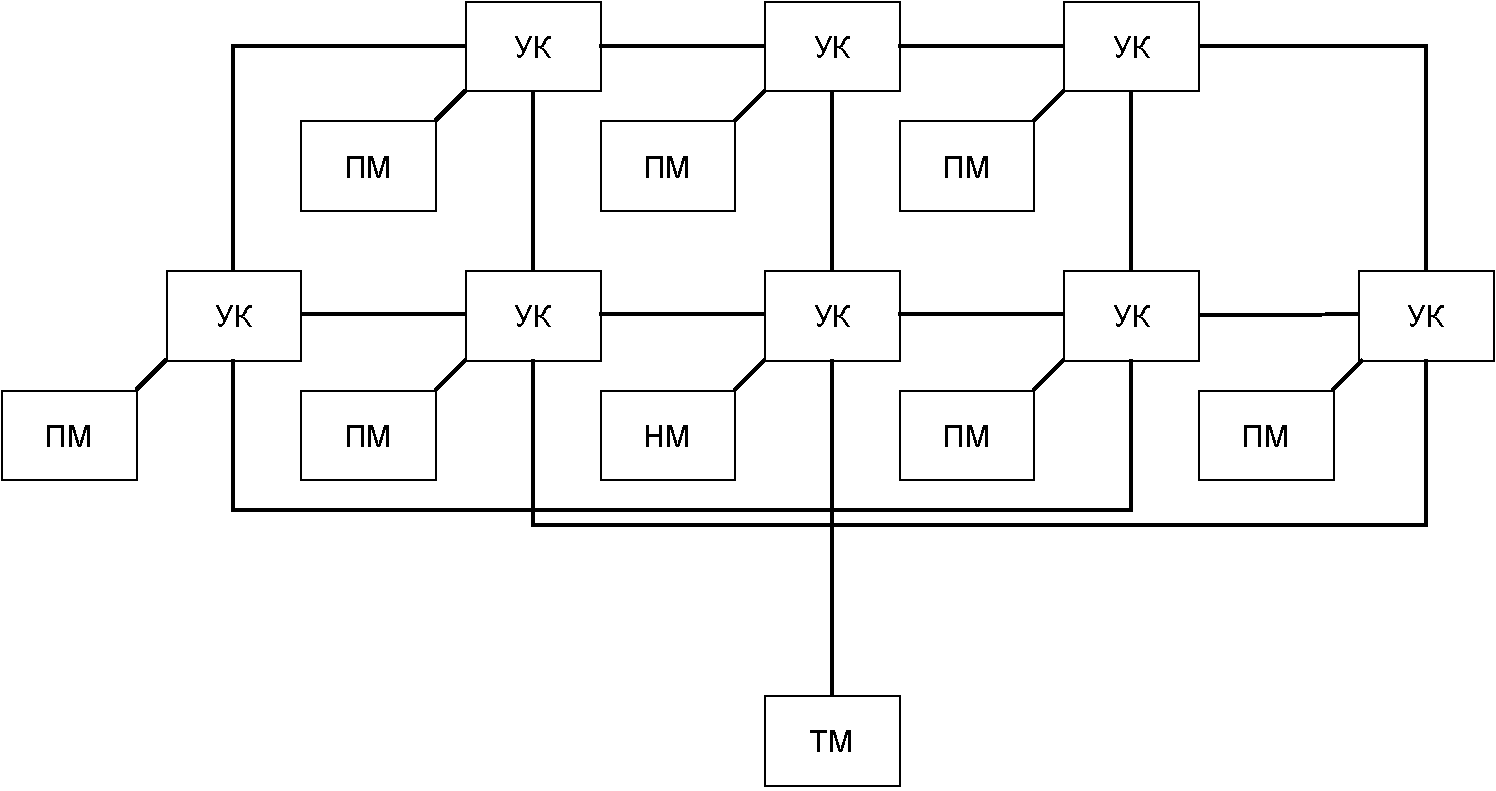
\includegraphics[scale=0.7]{images/part6/chapter_computer/coarse-grained architecture.pdf}
	\label{fig:coarse-grained-architecture}
\end{figure}

Основным достоинством крупнозернистой архитектуры \textit{ассоциативных семантических компьютеров} является ориентация на аппаратную поддержку параллельной обработки конструкций \textit{SC-кода}. В то же время у такого варианта реализации выделяется ряд недостатков:
\begin{textitemize}
	\item Каждый комбинированный модуль строится по принципам \textit{машины фон Неймана}, соответственно, ее недостатки в полной мере не устраняются;
	\item Несмотря на сохранение общих принципов \textit{SC-кода} и \textit{Языка SCP}, распределенное хранение и обработка sc-конструкций требует разработки отдельных языковых средств, таких как \textit{SCD-код} и \textit{Язык SCPD}, и их поддержки на базе выбранной аппаратной архитектуры. Кроме того, как видно и рассмотренных выше принципов \textit{Языка SCPD}, при разработке \textit{scpd-программ} необходимо явно учитывать тот факт, что обработка выполняется распределенно.
\end{textitemize}	

Следующий шагом с точки зрения иерархии архитектур \textit{ассоциативных семантических компьютеров} является мелкозернистая архитектура ассоциативных семантических компьютеров.

\subsection{Вариант мелкозернистой архитектуры ассоциативных семантических компьютеров}
\label{subsec_comp_fine}

Как уже было сказано, целесообразность перехода от крупнозернистых архитектур к мелкозернистым обусловлена  соответствующим увеличением степени потенциального параллелизма в процедурах переработки знаний. При этом максимально возможный параллелизм, очевидно, будет иметь место при предельной реализации мелкозернистых архитектур, в которых один структурный модуль процессоро-памяти будет соответствовать одному элементу памяти, то есть в нашем случае --- одному sc-элементу.

Рассмотрим более детально принципы, лежащие в основе мелкозернистой архитектуры \textit{ассоциативного семантического компьютера}:
\begin{textitemize}
	\item Процессоро-память \textit{ассоциативного семантического компьютера} состоит из однотипных модулей, которые будем называть процессорными элементами sc-памяти или просто \textit{процессорными элементами}. Каждый \textit{процессорный элемент} соответствует одному sc-элементу (хранит один sc-элемент). При этом в каждый момент времени каждый \textit{процессорный элемент} может быть пустым (не хранить никакой sc-элемент) или заполненным, то есть иметь взаимно однозначно соответствующий ему хранимый sc-элемент. На физическом уровне для описания этого факта вводится соответствующий признак, имеющим два значения. Таким образом, каждый \textit{процессорный элемент} "отвечает"{} только за один sc-элемент и, в отличие от крупнозернистого варианта архитектуры \textit{ассоциативного семантического компьютера}, \myuline{задача не может быть решена} \myuline{одним \textit{процессорным элементом}} и количество таких \textit{процессорных элементов} достаточно велико (соответствует максимальному возможному числу sc-элементов, хранимых в базе знаний некоторой ostis-системы). Опыт разработки прикладных ostis-систем показывает, что в среднем число sc-элементов в базе знаний такой ostis-системы составляет от нескольких сотен тысяч до нескольких миллионов. Ситуация, когда в рамках процессоро-памяти необходимо представить sc-конструкцию, число элементов которой больше числа \textit{процессорных элементов} на данный момент не рассматривается и требует дополнительного исследования.
	\item Каждый \textit{процессорный элемент} (по аналогии с ячейкой памяти в случае реализации \textit{ассоциативного семантического компьютера} на фон-Неймановской архитектуре) имеет некоторый уникальный внутренний идентификатор --- \textit{\myuline{адрес} процессорного элемента}. Адреса \textit{процессорных элементов}, в отличие от адресов ячеек фон-Неймановской памяти, \myuline{не обеспечивают непосредственный доступ} к \textit{процессорным элементам}, а позволяют однозначно \myuline{идентифицировать} процессорный элемент при обмене сообщениями согласно рассмотренным ниже принципам.
	\item Каждый процессорный элемент имеет память, в которой хранится
	\begin{textitemize}
		\item синтаксическая метка, задающая тип соответствующего sc-элемента;
		\item содержимое внутреннего файла ostis-системы или ссылка на внешнюю файловую систему (если данный процессорный элемент соответствует внутреннему файлу ostis-системы);
		\item перечень логических связей данного процессорного элемента с другими, то есть перечень адресов процессорных элементов, связанных с данным процессорным элементом \textit{логическими каналами связи} с указанием типа связи (подробнее о \textit{логических каналах связи} см. ниже);
		\item метка блокировки sc-элементов с указанием метки соответствующего процесса;
		\item другие метки при необходимости (например, метки уровня доступа к хранимому sc-элементу);
		\item волновые микропрограммы, выполняемые данным процессорным элементом в данный момент (подробнее о \textit{волновых микропрограммах} см. ниже), и временные данные для этих микропрограмм, а также очередь микропрограмм при необходимости.
	\end{textitemize}
	\item Процессорные элементы связаны между собой двумя типами каналов связи --- \textit{физическими каналами связи} и \textit{логическими каналами связи}. 
	\begin{textitemize}
		\item В общем случае число \textit{физических каналов связи} у каждого \textit{процессорного элемента} может быть произвольным, кроме того теоретически \textit{физические каналы связи} между процессорными элементами могут перестраиваться (перекоммутироваться) с течением времени, например, с целью оптимизации времени передачи сообщений между процессорными элементами. Конфигурация \textit{физических каналов связи} не учитывается на уровне логической обработки знаний, как на уровне Языка SCP, так и на уровне языка микропрограмм, обеспечивающих интерпретацию команд Языка SCP, то есть \textit{scp-операторов}. Для упрощения в рамках данной работы будем рассматривать вариант физической реализации sc-памяти, в котором каждый процессорный элемент имеет фиксированное и одинаковое для всех процессорных элементов число \textit{физических каналов связи} (N), при этом конфигурация таких каналов связи с течением времени не меняется. Очевидно, что минимальным значением N является 2, в этом случае мы получим линейную цепочку \textit{процессорных элементов}. При N равном 4 мы получим двумерную "матрицу"{} \textit{процессорных элементов}, При N равном 6 --- трехмерную "матрицу"{} \textit{процессорных элементов} и так далее. Будем называть ``смежными'' \textit{процессорные элементы}, непосредственно связанные \textit{физическим каналом связи}.
		\item В таком случае можно сказать, что каждый процессорный элемент имеет свой "адрес"{} (уникальный идентификатор) в некотором многомерном пространстве, число измерений (признаков) которого определяется числом N \textit{физических каналов связи}, связанных с одним \textit{процессорным элементом}. В приведенных выше примерах размерность такого пространства равна N/2, что позволяет предположить, что число N целесообразно делать четным.
		\item Каждый \textit{физический канал связи} и каждый \textit{логический канал связи}, таким образом, задается парой \textit{адресов процессорных элементов}.
		\item \textit{логические каналы связи} между процессорными элементами формируются динамически и соответствуют \textit{связям инцидентности} между sc-элементами. Таким образом, \textit{логические каналы связи} могут описывать два типа связей инцидентности --- \textit{инцидентность обозначений sc-пар с их компонентами} и \textit{инцидентность обозначений ориентированных sc-пар с их вторыми компонентами} (см. \textit{\ref{sec_syntactic_core_sc_code}~\nameref{sec_syntactic_core_sc_code}}). При этом конфигурация \textit{логических каналов связи} в общем случае никак не связана с конфигурацией \textit{физических каналов связи} --- инцидентные sc-элементы могут физически храниться в процессорных элементах, не являющихся смежными. В тоже время очевидно, что в общем случае некоторые \textit{физические каналы связи} могут соответствовать логическим.
		\item Кроме связей инцидентности \textit{логические каналы связи} могут соответствовать и другим типам связей между sc-элементами, по аналогии с тем, как это сделано в программном варианте реализации ostis-платформы (см. \textit{Главу \ref{chapter_soft_platform}~\nameref{chapter_soft_platform}}). Например, для упрощения реализации алгоритмов поиска в базе знаний и уменьшения объема памяти, которым должен обладать каждый \textit{процессорный элемент}, целесообразно хранить в памяти процессорного элемента адрес только первого sc-коннектора, инцидентного соответствующему sc-элементу соответствующим типом инцидентности, а в рамках процессорного элемента, соответствующего данному sc-коннектору, адрес следующего sc-коннектора, инцидентного тому же sc-элементу тем же типом инцидентности и так далее. При таком подходе количество памяти процессорного элемента, хранящей логические связи между процессорными элементами, можно сделать фиксированным.
	\end{textitemize}
	\item Каждый процессорный элемент может отправлять сообщения (микропрограммы) другим процессорным элементам и принимать сообщения от других процессорных элементов по \textit{логическим каналам связи} и имеет соответствующие рецепторно-эффекторные подмодули. На физическом уровне передача сообщений осуществляется, в свою очередь, по \textit{физическим каналам связи}, конфигурация которых, как было сказано выше, фиксируется и в общем случае не зависит от конфигурации логических каналов связи.
	\item Таким образом, процессорные элементы формируют однородную процессоро-память, в которой нет отдельно выделяемых модулей, предназначенных только для хранения информации и отдельно выделяемых модулей, предназначенных только для ее обработки. 
	\item Для связи такой процессоро-памяти с внешней средой вводится \textit{терминальный модуль}, который в общем случае может быть реализован по разному и задачами которого являются:
	\begin{textitemize}
		\item подготовка (генерация) информации, поступающей из внешней среды для ее последующей загрузки в процессорные модули;
		\item передача (использование, реализация) информации, подготовленной (полученной, представленной) в процессорных модулях, во внешнюю среду.
	\end{textitemize}
	\item Для хранения содержимых внутренних файлов ostis-системы большого размера может оказаться целесообразным иметь отдельную файловую память, связанную с процессоро-памятью и построенную по традиционным фон-Неймановским принципам. Это обусловлено тем, что основная цель построения процессоро-памяти -- обеспечение как можно большей параллельности при обработке конструкций SC-кода, в случае же с хранением и обработкой содержимых внутренних файлов ostis-системы, которые по определению являются внешними по отношению к SC-коду информационными конструкциями, целесообразно использовать современные традиционные подходы.
\end{textitemize}

Перечисленные принципы позволяют сформулировать ключевую особенность обработки информации, хранимой в рамках такой процессоро-памяти. В отличие от архитектуры фон-Неймана (и других архитектур, разработанных примерно в то же время, например, Гарвардской архитектуры) и даже от \textit{программного варианта ostis-платформы} в предлагаемой архитектуре процессоро-памяти \myuline{отсутствует общая память}, доступная для всех модулей, осуществляющих обработку информации. Благодаря этому значительно упрощается параллельная обработка информации, однако усложняется реализации набора микропрограмм интерпретации команд обработки информации в такой памяти, поскольку каждый процессорный элемент становится очень "близоруким"{} и "видит"{} только те процессорные элементы, которые связаны с ним \textit{логическими каналами связи}. 

Таким образом, язык описания микропрограмм интерпретации команд \textit{ассоциативного семантического компьютера} не может быть построен как традиционный язык программирования, например, процедурного типа, поскольку все такие языки предполагают возможность непосредственного адресного или ассоциативного доступа к произвольным элементам памяти. Предлагаемый язык описания микропрограмм предлагается строить по принципам \textit{волновых языков программирования} (см. \scncite{Sapatyj1986}, \scncite{Moldovan1985}) и инсерционного программирования (см. \scncite{Letichevskij2003}, \scncite{Letichevskij2012}).

В рамках такого языка микропрограмм выделяется два типа волн:
\begin{textitemize}
	\item Волны, передаваемые только по \textit{логическим каналам связи} (например, при поиске инцидентных sc-элементов).
	\item Волны, передаваемые по всем каналам связи (например, при создании новых логических каналов связи, то есть при генерации новых sc-элементов).
\end{textitemize}

Рассмотрим более детально принципы интерпретации команд (scp-операторов) в рамках рассмотренной процессоро-памяти.
\begin{textitemize}
	\item Каждый \textit{процессорный элемент} может интерпретировать некоторый ограниченный набор микропрограмм. С учетом того, что один процессорный элемент соответствует одному sc-элементу, то множество операций, связанных с преобразованием данного sc-элемента, очень ограничено (сгенерировать sc-элемент указанного типа, удалить sc-элемент, изменить содержимое sc-файла, установить или снять метку блокировки и так далее). Таким образом, важной задачей процессорного элемента будет формирование сообщений для других процессорных элементов и их отправка.
	\item Каждый процессорный элемент может порождать и хранить в памяти временные данные для микропрограмм. Предполагается, что объем памяти, имеющейся в распоряжении процессорного элемента, достаточен для представления всех необходимых данных для возможного набора микропрограмм, поскольку такие микропрограммы достаточно просты (см. предыдущий принцип). В случае, если по каким-либо причинам переполнение все же происходит, то могут использоваться различные подходы, например, описанные в работе \scncite{Kuzmickij2000}.
	\item Каждый процессорный элемент может сформировать микропрограмму и отправить ее в виде волнового сообщения для выполнения другими процессорными элементами. Передача сообщений происходит по физическим каналам связи. Поскольку конфигурация физических каналов связи в общем случае не связана конфигурацией логических каналов связи, то каждый процессорный элемент самостоятельно принимает решение о необходимости выполнения микропрограммы и передачи ее дальше. Здесь можно провести аналогию с волновым алгоритмом поиска пути в графе (вариант поиска в ширину).
	\item Часто процессорные элементы будут не выполнять микропрограмму, а передавать ее дальше, таким образом, сами процессорные элементы выполняют также и роль коммутационных элементов, при этом в общем случае каждый процессорный элемент может входить в произвольное число маршрутов при передаче сообщений по логическим каналам связи между процессорными элементами.
	\item Как и в случае с крупнозернистой архитектурой, у каждого процессорного элемента есть очередь микропрограмм, подлежащих выполнению (входящих сообщений), и очередь микропрограмм, подлежащих отправке (выходящих сообщений). При этом в рамках каждого процессорного элемента также можно говорить о возможности параллельного выполнения каких-либо операций (например, формирование выходящих сообщений и обработку текущего хранимого sc-элемента).
\end{textitemize}

Соответственно, можно говорить об иерархии микропрограмм:
\begin{textitemize}
	\item Микропрограммы по изменению хранимого sc-элемента:
	\begin{textitemize}
		\item Выполнить указанное преобразование содержимого данного sc-узла;
		\item Изменить метку типа sc-элемента (если такое изменение не противоречит \textit{Синтаксису SC-кода});
		\item Заменить блокировку данного sc-элемента для указанного процесса (в том числе, снять метку);
		\item Удалить sc-элемент.
	\end{textitemize}
	\item Микропрограммы по обработке sc-элементов, хранимых в других (не обязательно смежных процессорных элементах):
	\begin{textitemize}
		\item Сгенерировать инцидентный sc-коннектор (и новый \textit{логический канал связи}), возможно, вместе со смежным sc-элементом;
		\item Сгенерировать оба или один sc-элемент, соединяемые данным sc-коннектором
		\item Найти все sc-коннекторы (то есть адреса соответствующих им процессорных элементов) указанного типа, инцидентные данному sc-элементу указанным типом инцидентности;
		\item Найти sc-узлы, инцидентные данному sc-коннектору.
	\end{textitemize}
	\item Микропрограммы по управлению процессами выполнения других микропрограмм:
	\begin{textitemize}
		\item Переслать указанную микропрограмму для исполнения из данного процессорного элемента по всем \myuline{указанным} каналам (инцидентным sc-коннекторам указываемого типа) всем \myuline{смежным} sc-элементам указываемого типа;
		\item Дождаться выполнения микропрограмм указанного типа, порожденных указанным процессорным элементом и результат их выполнения передать процессорному элементу, запросившему соответствующую информацию.
	\end{textitemize}
	\item И другие
\end{textitemize}

Очевидно, что при решении конкретной задачи указанные микропрограммы могут комбинироваться в более сложные микропрограммы. Приведенная иерархия на данный момент не является полной и требует дальнейшего уточнения.

Исходя из представленных принципов формируется иерархия языков программирования для предложенной мелкозернистой архитектуры \textit{ассоциативных семантических компьютеров}:
\begin{textitemize}
	\item Язык SCP, не зависящий от реализации ostis-платформы, на котором пишутся программы sc-агентов обработки знаний. Язык SCP является "водоразделом"{} между платформенно-зависимой частью и платформенно-независимой частью ostis-системы, таким образом, он является самым низкоуровневым языком среди всех возможных платформенно-независимых языков, и одновременно языком высокого уровня с точки зрения ostis-платформы. 
	\item Язык микропрограмм, которыми обмениваются процессорные элементы между собой, и которые исполняются этими процессорными элементами. Фактически на этом языке разрабатывается интерпретатор Языка SCP. Важно отметить, что язык микропрограмм ориентирован на передачу сообщений по \textit{логическим каналам связи} и не учитывает конфигурацию \textit{физических каналов связи}. Для этого вводится еще один язык более низкого уровня.
	\item Язык для записи программ управления процессами обмена сообщениями (микропрограммами). Введение такого языка необходимо, поскольку, как было сказано, сам по себе язык микропрограмм не учитывает 
	\begin{textitemize}
		\item Конфигурацию физических каналов связи. Таким образом, при отправке сообщения по логическому каналу связи необходимо сформировать необходимое число сообщений в зависимости от числа имеющихся физических каналов связи, осуществить кодирование передаваемого сообщения для передачи по физическому каналу связи, передать сообщение с учетом того, что один и тот же физический канал связи может входить в общем случае в произвольное число маршрутов между процессорными элементами, осуществить декодирование сообщения на принимающем процессорном элементе. Все эти задачи требуют разработки соответствующих программ;
		\item Организацию очереди входящих и выходящих сообщений внутри \textit{процессорного элемента}, добавление сообщений в очередь, извлечение сообщений из очереди для выполнения и так далее.
	\end{textitemize}
\end{textitemize}

Достоинства предложенного мелкозернистого варианта архитектуры \textit{ассоциативных семантических компьютеров}:
\begin{textitemize}
	\item В рамках предложенной мелкозернистой архитектуры, в отличие от крупнозернистой, нет необходимости создания копий sc-элементов, и разработки специальных языков кодирования для полученных конструкция, таких как \textit{SCD-код}, поскольку каждый процессорный элемент хранит один атомарный фрагмент всей хранимой sc-конструкции и число логических связей с другими процессорными элементами не ограничено.
	\item Приведенная явно выделяемая иерархия языков программирования позволяет исключить на уровне разработки пользовательских программ (на \textit{Языке SCP} и языков более высокого уровня на его основе) необходимость учитывать факт распределенного хранения sc-конструкций и вообще принципы организации ostis-платформы. Другими словами, не требуется разработка таких языков, как \textit{Язык SCPD}.
	\item Расширяемость архитектуры позволяет легко наращивать число процессорных элементов без существенного снижения производительности, поскольку в предложенной архитектуре нет явно выделяемых процессорных модулей и накопительных модулей, соответственно исключается необходимость передачи информации между такими модулями, кроме того процессорный модуль перестает быть разделяемым ресурсом для большого числа одновременно выполняемых процессов. Все перечисленное позволит в конечном итоге решить проблему, известную как проблема "бутылочного горлышка"{} архитектуры фон Неймана (см. \scncite{Backus1978}).
	\item Ключевым достоинством предложенной мелкозернистой архитектуры является ее ориентация на максимально возможную поддержку параллельной обработки информации на аппаратном уровне и в конечном итоге возможность реализации \myuline{любых} моделей параллелизма с учетом решаемой задачи. В подтверждение данного тезиса можно привести теорию А-систем, описанную в работе В. Е. Котова и А. С. Нариньяни \scncite{Kotov1966}. По словам самих авторов, данное понятие стоит трактовать как универсальную модель для некоторого класса параллельных систем, которая требует уточнения в случае конкретных реализаций. В частности, в рамках данной теории выделяются процессорные элементы, активация/деактивация которых осуществляется посредством так называемой спусковой функции, принимающей значения 0 и 1. Понятно, что в конкретной реализации в качестве такой функции может быть использован любой признак, имеющий значения истина и ложь, указывающий на то, что тот или процессорный элемент должен быть активирован в следующий момент времени. Авторами показана возможность формализации на основе данной модели любых параллельных алгоритмов, рассмотрена возможность сведения таких алгоритмов к последовательным, варианты синхронизации в рамках такой модели. 
	
	Можно провести очевидную параллель между А-системами и предложенной мелкозернистой архитектурой \textit{ассоциативных семантических компьютеров} с учетом наличия волнового языка микропрограммирования:
	\begin{textitemize}
		\item Процессорным элементам из теории А-систем соответствуют \textit{процессорные элементы} процессоро-памяти;
		\item В роли спусковых функций для процессорных элементов выступают микропрограммы, передаваемые волнами от одного процессорного элемента к другому и, соответственно, активизирующие деятельность процессорных элементов.
	\end{textitemize}

	Стоит отметить, что несмотря на то, что рассмотренная работа по теории А-систем известна уже более полувека, авторам данной главы не удалось найти попытки реализовать идеи этой теории в аппаратном варианте. На наш взгляд, это обусловлено тем, что уровень развития микроэлектроники на тот момент не соответствовал необходимым для реализации теории А-систем требованиям.
\end{textitemize}

Вместе с перечисленными достоинствами можно выделить ключевой недостаток предложенного мелкозернистого варианта архитектуры \textit{ассоциативных семантических компьютеров}, который заключается в сильной зависимости быстродействия процессоро-памяти от времени передачи волновых микропрограмм от одного процессорного элемента к другому. При этом, поскольку на логическом уровне передача сообщений осуществляется по \textit{логическим каналам связи}, а реально --- по \textit{физическим каналам связи}, то быстродействие процессоро-памяти будет зависеть от того, насколько близко соответствует конфигурация \textit{логических каналов связи} конфигурации \textit{физических каналов связи}. Очевидно, что в общем случае взаимно однозначное соответствие этих конфигураций невозможно, поскольку число \textit{физических каналов связи}, инцидентных заданному процессорному элементу, ограничено в отличие от числа \textit{логических каналов связи}. Тем не менее, возможны несколько вариантов оптимизации размещения sc-конструкций в процессоро-памяти:
\begin{textitemize}
	\item при записи ("укладке"{}) sc-конструкции в процессоро-память (в особенности в случае достаточно больших sc-конструкций) можно учитывать \myuline{семантику} записываемых фрагментов, и записывать их таким образом, чтобы те sc-элементы, сообщение к которым будет передаваться от данного sc-элемента с большей вероятностью, находились физически ближе к данному sc-элементу. Так, например, можно учитывать денотационную семантику scp-операторов поиска, которые ориентированы на обработку \textit{трехэлементных sc-конструкций} и \textit{пятиэлементных sc-конструкций}, а также хранить sc-элементы, инцидентные заданному sc-коннектору по возможности ближе к нему;
	\item Если число логических связей между элементами sc-конструкции не превышает числа доступных физических каналов связи процессорного элемента и sc-граф является планарным (хоть sc-граф не является классическим графом, можно говорить о его планарности по аналогии с планарностью классических графов), то возможна запись sc-конструкции в процессоро-память таким образом, чтобы конфигурация \textit{логических каналов связи}  взаимно однозначно соответствовала какому-то подмножеству физических каналов связи. Таким образом, актуальной является разработка алгоритмов оптимальной "укладки"{} sc-графов в процессоро-память для обеспечения последующей эффективности передачи сообщений между процессорными элементами;
	\item Поскольку конфигурация \textit{логических каналов связи} меняется в процессе обработки sc-конструкций, то целесообразно говорить также о разработке алгоритмов переразмещения ("дефрагментации") уже записанной в процессоро-память sc-конструкции с целью обеспечения последующей эффективности передачи сообщений. Такое переразмещение может выполняться, например, по расписанию в период, когда процессоро-память не используется для решения других задач;
	\item Кроме того, при наличии аппаратной возможности может выполняться также перекоммутация \textit{физических каналов связи} с целью приближения их конфигурации к конфигурации \textit{логических каналов связи}.
\end{textitemize}

Рассмотрим пример оптимального варианта записи простейшей \textit{пятиэлементной sc-конструкции} в предлагаемую процессоро-память в рамках мелкозернистой архитектуры \textit{ассоциативных семантических компьютеров}.

На рисунке \textit{\nameref{fig:computer-graph1}} показана запись некоторой \textit{пятиэлементной sc-конструкции} в SCg-коде.

\begin{figure}[H]
	\caption{SCg-текст. Пример \textit{пятиэлементной sc-конструкции}}
	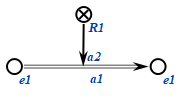
\includegraphics[scale=0.8]{images/part6/chapter_computer/computer graph1.png}
	\label{fig:computer-graph1}
\end{figure}

На рисунке \textit{\nameref{fig:incidence-example}} показан граф инцидентности для той же \textit{пятиэлементной sc-конструкции}, который позволяет свести sc-конструкцию к классическому графу с двумя типами связей. Для наглядности синтаксические типы соответствующих sc-элементов на рисунке не показаны.

\begin{figure}[H]
	\caption{Рисунок. Граф инцидентности для \textit{пятиэлементной sc-конструкции}}
	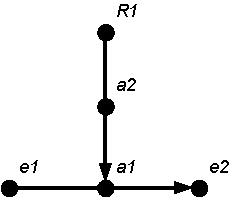
\includegraphics[scale=1]{images/part6/chapter_computer/incidence example.pdf}
	\label{fig:incidence-example}
\end{figure}

На рисунке \textit{\nameref{fig:fine-grained-architecture}} показан один из возможных оптимальных вариантов записи полученного графа инцидентности в процессоро-память. Пунктирными линиями показаны \textit{физические каналы связи} между процессорными элементами, сплошными --- \textit{физические каналы связи}, соответствующие \textit{логическим каналам связи}. Отметим, что элемент \textbf{\textit{R1}} целесообразно записать в \textit{процессорный элемент}, соседний с \textit{процессорным элементом}, хранящим элемент \textbf{\textit{e1}} или элемент \textbf{\textit{e2}}, как и показано на рисунке. Благодаря этому процессорные элементы, хранящие указанные sc-элементы, оказываются непосредственно связаны \textit{физическим каналом связи}, что упрощает коммуникацию в случае рассылки сообщений по \textit{физическим каналам связи} без учета \textit{логических каналов связи}.

\begin{figure}[H]
	\caption{Рисунок. Пример укладки sc-конструкции в процессоро-память}
	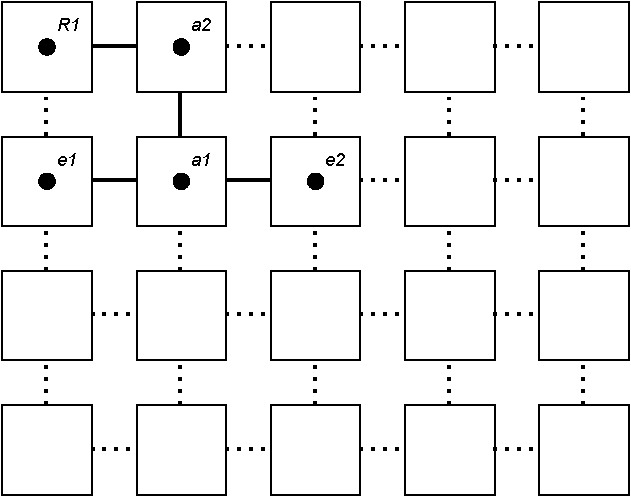
\includegraphics[scale=1]{images/part6/chapter_computer/fine-grained architecture.pdf}
	\label{fig:fine-grained-architecture}
\end{figure}

\section*{Заключение к Главе \ref{chapter_computers}}
В главе рассмотрены недостатки доминирующей в настоящее время фон-Неймановской архитектуры компьютерных систем в качестве основы для построения интеллектуальных компьютерных систем нового поколения, проведен анализ современных подходов к разработке аппаратных архитектур, устраняющих некоторые из указанных недостатков, обоснована необходимость разработки принципиально новых аппаратных архитектур, представляющих собой аппаратный вариант реализации ostis-платформ --- \textit{ассоциативных семантических компьютеров}.

Предложены общие принципы, лежащие в основе \textit{ассоциативных семантических компьютеров}, рассмотрены три возможных варианта архитектуры таких компьютеров, представлены их достоинства и недостатки.

Дальнейшее развитие предложенных в главе подходов требует решения ряда задач, как технических, так и организационных:
\begin{textitemize}
	\item Разработка волнового языка для записи микропрограмм, которыми обмениваются процессорные элементы между собой, и которые исполняются этими процессорными элементами;
	\item Разработка языка для записи программ управления процессами обмена микропрограммами и управления очередью микропрограмм;
	\item Организация активного участия специалистов в области микроэлектроники в уточнении принципов реализации процессорных элементов и процессоро-памяти в целом, уточнение элементной базы и более низкоуровневых архитектурных особенностей \textit{ассоциативных семантических компьютеров};
	\item Разработка алгоритмов оптимизации способов записи sc-конструкций в процессоро-память и переразмещения уже записанной sc-конструкции с целью обеспечения последующей эффективности передачи сообщений между процессорными элементами;
	\item Уточнение типологии информационных процессов в процессоро-памяти, их свойств и соответствующей типологии меток;
	\item Уточнение принципов реализации многоагентной обработки знаний в рамках процессоро-памяти, в частности, разработка принципов реализации событийной обработки информации в такой памяти.
\end{textitemize}
